\documentclass[a4paper,12pt]{article}
\usepackage[utf8]{inputenc}
\usepackage[ngerman]{babel}
\usepackage[T1]{fontenc}
\usepackage[scaled]{uarial}
\usepackage{amsmath}
\usepackage{titling}
\usepackage{fancyhdr}
\usepackage{calc}
\usepackage[a4paper, margin=2.5cm]{geometry}
\usepackage{tocloft}
\usepackage{graphicx}
\usepackage{caption}
\usepackage{acronym}
\usepackage{upquote}
\usepackage[style=authoryear,backend=biber]{biblatex}
\addbibresource{Quellen.bib}
\usepackage{csquotes}
\usepackage{filecontents}
\usepackage{setspace}
\usepackage{ragged2e}
\usepackage{framed}
\usepackage{tabularx}
\usepackage{geometry}
\usepackage{fancyhdr}
\usepackage{enumitem}
\usepackage[parfill]{parskip}
\usepackage{float}
\usepackage{etoolbox}
\usepackage{booktabs}
\usepackage{mdframed}
\usepackage[table]{xcolor}
\usepackage{amsmath, amssymb}
\geometry{a4paper, margin=2.5cm}
\usepackage[version=4]{mhchem}
\usepackage{textcomp}
\DeclareUnicodeCharacter{2082}{$_2$}
\DeclareUnicodeCharacter{00B1}{\ensuremath{\pm}}
\usepackage{listings}
\usepackage{xcolor}




\setlength\bibnamesep{1.5\itemsep}
\renewcommand{\cftsecleader}{\cftdotfill{\cftdotsep}}
\linespread{1.5}
\pagestyle{fancy}
\renewcommand*\familydefault{\sfdefault}
\fancyhf{}
\setlength{\parskip}{6pt}
\onehalfspacing
\justifying
\fancyhead[L]{Einsatz von GenAI-Technologien zur Bewertung von Antworten}
\cfoot{\tiny Studienarbeit / Stand \today \hfill \thepage}
\title{Einsatz von GenAI-Technologien zur Bewertung von Antworten}
\author{Len Vejsada}
\date{19. Mai 2025}
\geometry{a4paper, margin=1in}
\setlength{\parindent}{0pt}


\renewcommand{\maketitle}{
  \begin{center}
    {\LARGE\textbf{\thetitle}}\\[2em]
    {{Studienarbeit\\[2em]
     des Studiengangs Informatik\\[0.5em]
     an der \\[0.5em]
     Dualen Hochschule Baden-Württemberg Karlsruhe\\[0.5em]
     von}}\\[1em]
    \theauthor\\[1em]
    \thedate\\[7em]
  \end{center}
}

\fancypagestyle{firstpage}{
  \fancyhf{}
  \renewcommand{\headrulewidth}{0pt}
  \cfoot{\tiny Studienarbeit / Stand \today \hfill \thepage}
}


\begin{document}
\pagenumbering{gobble}
\pagenumbering{roman}
\setcounter{page}{1}
\thispagestyle{firstpage}
\begin{figure}
\begin{center}
  
\includegraphics[width=\textwidth]{Bilder/KardexRemstar.png}
  \label{fig:logo}
\end{center}
\end{figure}
  
\maketitle

\begin{tabular}{l@{\hspace{2em}}l}
  Matrikelnummer & 9447853 \\[0.5em]
  Kurs & TINF22B6 \\[0.5em]
  Ausbildungsfirma & Kardex, Bellheim \\[0.5em]
  Betreuer & Simon Franke \\[0.5em]
\end{tabular}

\newpage

\textbf{Genderhinweis} \\
Aus Gründen der leichteren Lesbarkeit wird in der vorliegenden Studienarbeit einheitlich die männliche Form verwendet. Diese bezieht zugleich weibliche als auch andere Geschlechtsidentitäten ein. \\



\thispagestyle{firstpage}
\textbf{Erklärung} \\
(gemäß §5(3) der „Studien- und Prüfungsordnung DHBW Technik“ vom
29. 9. 2015)
Ich versichere hiermit, dass ich meine Studienarbeit mit dem Thema: „Einsatz von GenAI-Technologien zur Bewertung von Antworten“ selbstständig verfasst und keine anderen als die angegebenen Quellen und Hilfsmittel benutzt habe. Ich versichere zudem, dass die eingereichte elektronische Fassung mit der gedruckten Fassung übereinstimmt.\\[1.5em]
\vspace{1cm}

\begin{center}
\begin{tabularx}{\textwidth}{X r}
Lustadt, 19.05.2025 & gez. Len Vejsada \\
\hline
\end{tabularx}
\end{center}

\noindent {\small Ort, Datum \hfill Unterschrift}\\

\newpage
\tableofcontents
\thispagestyle{fancy}
\thispagestyle{firstpage}
\newpage

\addcontentsline{toc}{section}{Abbildungsverzeichnis}
\listoffigures

\newpage
\listoftables
\addcontentsline{toc}{section}{Tabellenverzeichnis}
\newpage
\section*{Abkürzungsverzeichnis}
\addcontentsline{toc}{section}{Abkürzungsverzeichnis}
\begin{acronym}
  \acro{CSharp}[C\#]{C Sharp}
  \acro{HTML}{Hypertext Markup Language}
  \acro{CSS}{Cascading Style Sheets}
  \acro{SCSS}{Sassy Cascading Style Sheets}
  \acro{SQL}{Structured Query Language}
  \acro{JS}{JavaScript}
  \acro{.NET}{Domain Network}
  \acro{ASP.NET}{Active Server Pages .NET}
  \acro{EF}{Entity Framework}
  \acro{ORM}{Object-Relational Mapping}
  \acro{API}{Application Programming Interface}
  \acro{SPA}{Single-Page Application}
  \acro{MPA}{Multi-Page Application}
  \acro{UI}{User Interface}
  \acro{DI}{Dependency Injection}
  \acro{TS}{TypeScript}
  \acro{SOA}{Service-Oriented Architecture}
  \acro{REST}{Representational State Transfer}
  \acro{MVP}{Minimum Viable Products}
  \acro{NLP}{Natural Language Processing}
  \acro{KI}{Künstliche Intelligenz}
  \acro{GPT}{Generative Pre-trained Transformer}
  \acro{SRS}{Software Requirements Specification}
  
  
\end{acronym}

\newpage

\pagenumbering{arabic}
\setcounter{page}{1}

\section{Ziele des Dokuments}
Ziel dieses Dokuments ist es, die Anforderungen, Zielsetzungen und den Kontext der entwickelten Softwarelösung systematisch darzustellen. Es beschreibt das konzeptionelle Fundament sowie die technischen und funktionalen Rahmenbedingungen des Projekts zur Bewertung von Antworten mit Hilfe generativer KI-Technologien. Das Dokument dient als Grundlage für Designentscheidungen, die technische Umsetzung und die spätere Evaluierung. Darüber hinaus schafft es Transparenz über den Umfang des Projekts und stellt sicher, dass alle Beteiligten ein einheitliches Verständnis des Projektziels und seiner Umsetzung gewinnen.

\section{Anlass und Motivation des Projekts}
Die Bewertung von offenen Antworten stellt nach wie vor eine erhebliche Herausforderung in digitalen Lernumgebungen dar. Während klassische Systeme auf einfache Mustererkennung und statische Entscheidungsregeln setzen, scheitern sie häufig daran, die Vielfalt korrekter Formulierungen adäquat zu erfassen. Bei Freitextantworten oder leicht abweichenden Formulierungen werden korrekte Inhalte häufig als inkorrekt eingestuft. Diese Einschränkungen wirken sich negativ auf die Fairness und Akzeptanz solcher Systeme aus.

Das vorliegende Projekt adressiert dieses Defizit durch die Integration generativer KI-Technologien, welche die Fähigkeit besitzen, Antworten kontextbasiert zu analysieren und flexibler zu bewerten. Ziel ist die Entwicklung eines Minimum Viable Product (MVP), das in der Lage ist, verschiedene Fragetypen zu verarbeiten und Antworten präzise zu bewerten, unabhängig von formalen Abweichungen wie Groß-/Kleinschreibung, Synonymen oder Tippfehlern. Durch den Einsatz einer serviceorientierten Webarchitektur soll eine modulare, erweiterbare Plattform entstehen, die sowohl für Bildungseinrichtungen als auch für Lernplattformen von Interesse ist. Die Ergebnisse dieser Arbeit können darüber hinaus als Grundlage für zukünftige Forschung zur adaptiven Lernpfadsteuerung oder multimodalen Antwortverarbeitung dienen.

\newpage

\section{Aufbau der Arbeit}
Die Arbeit beginnt mit einer theoretischen Fundierung des Themas und der Einordnung generativer KI-Technologien im Kontext automatisierter Antwortbewertung. Darauf aufbauend wird die Zielsetzung des Projekts beschrieben und die Konzeption des entwickelten Prototyps erläutert. Im Anschluss erfolgt eine detaillierte Darstellung der technischen Architektur, der eingesetzten Technologien sowie der zugrunde liegenden Systemlogik. Es folgt eine Beschreibung der konkreten Implementierungsschritte, einschließlich der Integration der Bewertungslogik und der Gestaltung der Benutzeroberfläche. Ein weiterer Schwerpunkt liegt auf der Analyse und Bewertung verschiedener GenAI-Ansätze hinsichtlich ihrer Leistungsfähigkeit, Genauigkeit und Kosteneffizienz. Abschließend werden die zentralen Ergebnisse zusammengefasst, Entwicklungserfahrungen reflektiert und mögliche Perspektiven für eine zukünftige Weiterentwicklung aufgezeigt.

\newpage

\section{Projektbeschreibung}
Die automatisierte Bewertung von Antworten stellt ein zentrales Element in digitalen Lernumgebungen dar. Um diese Herausforderung angemessen zu adressieren, zielt das vorliegende Projekt auf die Entwicklung eines innovativen Bewertungssystems, das generative KI-Technologien nutzt, um die Genauigkeit und Flexibilität der Auswertung zu verbessern. Die folgenden Abschnitte beschreiben die Zielsetzung, den konzeptionellen Aufbau sowie die Abgrenzung des entwickelten MVPs.


\subsection{Projektziele}
Im Zentrum des Projekts steht die Entwicklung eines webbasierten Systems, das generative KI nutzt, um Antworten in digitalen Lernumgebungen kontextsensitiv und tolerant gegenüber sprachlichen Abweichungen zu bewerten. Dies umfasst insbesondere die Fähigkeit, unterschiedliche Antwortformate, Synonyme sowie orthografische Abweichungen zu erkennen und in die Bewertung einzubeziehen.

Über die isolierte Analyse einzelner Antworten hinaus sollen Nutzer die Möglichkeit erhalten, vollständige Prüfungen zu erstellen, bestehend aus individuell konfigurierbaren Fragetypen. Diese Prüfungen können online bearbeitet werden; nach ihrer Abgabe erfolgt die automatisierte Auswertung durch ein angebundenes generatives KI-Modul auf Basis der OpenAI-API. Diese API ermöglicht eine semantische Analyse der Antworten und generiert differenzierte Bewertungen inklusive punktgenauer Rückmeldungen.

Die Ergebnisse werden den Teilnehmenden unmittelbar nach der Auswertung zur Verfügung gestellt. Zusätzlich erhalten sie Zugang zu persönlichen Ergebnisübersichten sowie zu statistischen Auswertungen, die den individuellen Lernfortschritt über verschiedene Prüfungsdurchläufe hinweg abbilden. Dadurch wird ein kontinuierliches, datenbasiertes Lernen unterstützt.

Ein weiteres Ziel ist der Aufbau einer modularen und erweiterbaren Softwarearchitektur, die zukünftige Erweiterungen, wie adaptive Lernpfade, multimodale Antwortverarbeitung oder differenzierte Bewertungsstrategien, ermöglicht. Die technische Umsetzung legt besonderen Wert auf Wartbarkeit, Skalierbarkeit und die klare Trennung von Verantwortlichkeiten innerhalb der Systemkomponenten.

\subsection{Überblick über das Minimum Viable Product (MVP)}
Das entwickelte MVP stellt eine funktionale Webanwendung dar, die auf einer modernen, komponentenbasierten Systemarchitektur basiert. Die Benutzeroberfläche wurde mit Angular umgesetzt und ermöglicht eine interaktive Verwaltung von Fragen, Prüfungsszenarien und Auswertungsergebnissen. Das Backend basiert auf ASP.NET Core und bietet über REST-APIs eine standardisierte Schnittstelle für die Kommunikation mit dem Frontend.

Die zentrale Funktionalität besteht in der automatisierten Bewertung von Antworten durch eine angebundene OpenAI-Komponente. Diese analysiert eingereichte Antworten unter Berücksichtigung definierter Bewertungskriterien wie Groß- und Kleinschreibung, semantischer Ähnlichkeit oder zulässiger Abweichung bei Schätzfragen. Dabei können Nutzer individuelle Einstellungen wie Toleranzlevel oder Genauigkeitsgrad festlegen, um die Bewertung an spezifische Anforderungen anzupassen.

Neben der Bewertungslogik umfasst das MVP auch eine persistente Datenhaltung über eine relationale Datenbank, in der alle relevanten Informationen zu Fragen, Nutzereingaben, Bewertungen und Einstellungen gespeichert werden. Eine integrierte Teststruktur stellt die funktionale Stabilität des Systems sicher und erleichtert künftige Erweiterungen.

\subsection{Abgrenzung und Einschränkungen}
Das entwickelte MVP verfolgt das Ziel, eine funktionsfähige Kernlösung bereitzustellen, die den Einsatz generativer KI für die automatisierte Bewertung in Lernsystemen demonstriert. Der Fokus liegt auf der technischen Realisierbarkeit sowie auf dem didaktischen Potenzial kontextsensitiver Antwortanalysen durch KI-gestützte Verfahren.

Auf erweiterte Funktionalitäten wie ein differenziertes Rollen- und Rechtemanagement wurde im aktuellen Entwicklungsstand verzichtet. Ein solches System, das zwischen Administratoren, Lehrkräften und Lernenden unterscheidet, stellt in produktiven Lernplattformen eine wichtige Grundlage für eine sichere und zielgruppenspezifische Nutzung dar. Im vorliegenden Prototyp wurde diese Funktion bewusst ausgeklammert, lässt sich jedoch mit geringem Entwicklungsaufwand ergänzen und bietet eine sinnvolle Erweiterung für zukünftige Versionen.

Auch auf umfassende Mehrsprachigkeit sowie die Einbindung alternativer Eingabeformen, wie Sprache oder Bilddaten, wurde verzichtet, um den Fokus auf die Kernfunktion der KI-gestützten Bewertung zu legen.

Die Bewertungslogik konzentriert sich im derzeitigen Entwicklungsstand auf grundlegende Kriterien wie Rechtschreibung, semantische Ähnlichkeit und Synonymtoleranz. Erweiterte Konzepte, wie adaptive Gewichtungen von Antworten, dynamische Bewertungsschemata oder eine Lernpfadsteuerung basierend auf individuellen Fortschrittsdaten, sind nicht Bestandteil des Prototyps.

Ein weiterer zentraler Aspekt der Abgrenzung betrifft die Bewertung selbst: Die eingesetzte OpenAI-API liefert zwar bemerkenswert leistungsfähige und flexible Analysen, bringt jedoch auch inhärente Unsicherheiten mit sich. Dazu zählen eine begrenzte Nachvollziehbarkeit der Bewertungsentscheidung, gelegentliche Inkonsistenzen sowie eine nicht deterministische Ergebnisstruktur \parencite{openai_reasoning}. Diese Eigenschaften sind technologisch bedingt und stellen eine Herausforderung dar, wenn es um die Reproduzierbarkeit und Objektivierbarkeit von Bewertungen geht. Die Interpretation und Einordnung der Bewertungsergebnisse erfordern daher ein reflektiertes Verständnis der Funktionsweise generativer Modelle \parencite{luckin}.

Trotz dieser Einschränkungen bietet das MVP eine tragfähige Grundlage für weiterführende Entwicklungen und zukünftige Forschungsfragen im Bereich KI-gestützter Lernsysteme.

\newpage

\section{Hintergrund und Kontext}
\label{sec:hintergrund}
Die digitale Transformation der Bildungslandschaft schreitet stetig voran und bringt tiefgreifende Veränderungen in der Art und Weise mit sich, wie Lehrinhalte vermittelt, erlernt und bewertet werden. Die Bewertung offener Antworten, beispielsweise bei Freitextaufgaben, stellt eine der anspruchsvollsten Herausforderungen in digitalen Lernumgebungen dar. Klassische regelbasierte Verfahren stoßen hier rasch an ihre Grenzen, da sie semantische Ähnlichkeiten, kontextuelle Bedeutungen und sprachliche Varianten nur unzureichend erfassen können. Um diese Limitationen zu überwinden, rücken generative KI-Technologien in den Fokus der Forschung und praktischen Anwendung \parencite{luckin}.

Die Leistungsfähigkeit dieser Technologien eröffnet neue Perspektiven für eine flexible, faire und individualisierte Bewertung von Antworten. Gleichzeitig sind jedoch auch neue Risiken und Verantwortlichkeiten entstanden. So können generative KI-Systeme, trotz ihrer beeindruckenden Sprachverarbeitungskapazitäten, inhaltlich fehlerhafte, irreführende oder unvollständige Aussagen erzeugen, ein Phänomen, das als „Halluzination“ bezeichnet wird. Darüber hinaus sind die Ergebnisse dieser Systeme nicht deterministisch, d.h. identische Eingaben können zu unterschiedlichen Ausgaben führen. Diese Eigenschaften stellen bei der automatisierten Bewertung von Prüfungsleistungen ein ernstzunehmendes Problem dar, insbesondere im Hinblick auf Reproduzierbarkeit, Nachvollziehbarkeit und pädagogische Fairness \parencite{openai_reasoning, luckin}.

Daher ist bei jeder Interaktion mit generativen KI-Systemen ein kritisches Bewusstsein erforderlich. Wie bereits bei der Nutzung von vielen Sprachmodell-basierten KIs ervorgehoben wird, muss man sich bewusst sein, dass menschenzentrierte Kontrolle und Reflexion weiterhin unverzichtbare Bestandteile jedes KI-gestützten Systems bleiben müssen. Wie auch in der Diskussion um KI in der Bildung betont wird, sind „Verantwortung, Transparenz, Nachvollziehbarkeit, Unbestechlichkeit und Vorhersehbarkeit [...] alles Kriterien, die bei einem Algorithmus berücksichtigt werden müssen, der menschliches Urteilsvermögen in sozialen Funktionen ersetzen soll“ \parencite[39]{luckin}. Auch im Rahmen dieses Projekts, das auf der Anbindung der OpenAI-API basiert, ist es essenziell, den von der KI generierten Bewertungen mit kritischer Distanz zu begegnen und sie nicht unreflektiert als endgültig oder fehlerfrei zu übernehmen. Eine sorgfältige Überprüfung durch fachkundige Personen bleibt unerlässlich, um Verzerrungen, Ungenauigkeiten oder kontextuelle Fehlinterpretationen zu erkennen und zu korrigieren. \parencite{luckin}

\newpage

\subsection{Technischer Hintergrund}
Die automatisierte Bewertung von Antworten in digitalen Lernumgebungen erfordert technologische Ansätze, die in der Lage sind, Sprache in all ihrer Komplexität zu verarbeiten. Traditionelle Methoden basieren auf regelbasierten Algorithmen, die durch Pattern Matching, statische Entscheidungsregeln oder gewichtete Punktesysteme operieren. Diese Ansätze sind zwar in bestimmten Szenarien effektiv, beispielsweise bei Multiple-Choice- oder numerischen Rechenfragen, stoßen jedoch bei offenen, natürlichsprachlichen Antworten an ihre Grenzen. Insbesondere bei Freitextantworten, bei denen Formulierungen variieren und semantische Ähnlichkeiten schwer algorithmisch greifbar sind, zeigen diese Methoden systematische Schwächen \parencite{jurafsky}.

Mit dem Aufkommen neuronaler Netzwerke und insbesondere transformerbasierter Sprachmodelle wurde eine neue Ära in der Verarbeitung natürlicher Sprache (Natural Language Processing, NLP) eingeläutet. Die sogenannte Generative Künstliche Intelligenz (Generative AI oder GenAI) beruht auf tiefen neuronalen Netzen, die in der Lage sind, Sprache nicht nur zu analysieren, sondern eigenständig zu generieren. Grundlage hierfür bilden umfangreiche Trainingsdaten aus Textkorpora sowie Mechanismen wie Selbstaufmerksamkeit, Positionskodierung und Fine-Tuning (vgl.  \textcite{radford}).

Ein zentrales Element dieser Technologie ist das Sprachmodell GPT (Generative Pre-trained Transformer), welches auf der Transformer-Architektur basiert (vgl. \textcite{vaswani2017attention}). Modelle wie GPT-3.5 oder GPT-4 von OpenAI wurden mit Milliarden von Textfragmenten trainiert, um syntaktische, semantische und kontextuelle Muster zu erkennen und zu reproduzieren. Diese Modelle operieren probabilistisch: Für jeden nächsten Token berechnet das Modell Wahrscheinlichkeiten, basierend auf dem bisherigen Eingabekontext. Das bedeutet, dass dieselbe Eingabe in leicht variierter Umgebung zu unterschiedlichen Ausgaben führen kann, ein Phänomen, das als Nichtdeterminismus bekannt ist (vgl. \textcite{openai_reasoning}).

Technisch betrachtet, führt dies zu einer fundamentalen Eigenschaft generativer KI: Sie ist nicht deterministisch und liefert keine garantierte Reproduzierbarkeit. Selbst bei identischem Prompt können Ausgaben variieren, weil intern stochastische Sampling-Mechanismen wie Top-k oder Temperatursteuerung zur Anwendung kommen \parencite{holtzman}. Darüber hinaus können generative Modelle auch Halluzinationen erzeugen, das heißt, sie liefern Aussagen, die inhaltlich falsch oder faktisch nicht belegbar sind, obwohl sie sprachlich korrekt erscheinen \parencite{openai_reasoning}. Diese Problematik stellt insbesondere bei der Bewertung von Lernleistungen eine erhebliche Herausforderung dar, da sie die Objektivierbarkeit, Nachvollziehbarkeit und Gerechtigkeit der Bewertung unterminieren kann.

Die technische Architektur eines GenAI-gestützten Bewertungssystems muss daher nicht nur die Interaktion zwischen Frontend, Backend und externem KI-Dienst ermöglichen, sondern auch Mechanismen zur Absicherung, Nachverfolgung und Parametrisierung der Bewertungsergebnisse implementieren. Die in diesem Projekt entwickelte Lösung basiert auf einer serviceorientierten Webarchitektur, die Angular für das Frontend und ASP.NET Core für das Backend einsetzt. Die Kommunikation mit der KI erfolgt über RESTful APIs und die OpenAI-API, wobei strukturierte Prompts genutzt werden, um konsistente Bewertungsanweisungen an das Modell zu übermitteln.


\subsection{Generative KI-Technologien: Definition und Bedeutung}
Der Begriff „Generative Künstliche Intelligenz“ (GenAI) bezeichnet eine Klasse von Algorithmen, die in der Lage sind, neue Inhalte zu erzeugen, die strukturell oder semantisch bestehenden Daten ähneln. Diese Inhalte können Texte, Bilder, Audiosequenzen oder andere komplexe Datenformen umfassen. Im Gegensatz zu traditionellen KI-Verfahren, die primär auf Klassifikation, Regression oder Entscheidungsbäumen beruhen, zielen generative Modelle darauf ab, neue Datenpunkte aus einem erlernten Wahrscheinlichkeitsraum zu erzeugen \parencite{mitkov}.

Zentraler technischer Motor generativer KI sind sogenannte Transformer-Architekturen, welche erstmals 2017 durch das „Attention is All You Need“-Paper von \textcite{vaswani2017attention} eingeführt wurden (vgl. Abb.~\ref{fig:transformer}). Diese Modelle nutzen Selbstaufmerksamkeitsmechanismen (vgl. \textcite{vaswani2017attention}), um komplexe Abhängigkeiten in Sequenzdaten wie natürlicher Sprache zu modellieren. Auf dieser Basis entwickelte Sprachmodelle wie GPT-3, GPT-3.5 oder GPT-4 (Generative Pre-trained Transformer) sind in der Lage, auf Basis eines gegebenen Kontexts plausible und kohärente Fortsetzungen, Antworten oder Erklärungen zu generieren.

\begin{figure}[H]
    \centering
    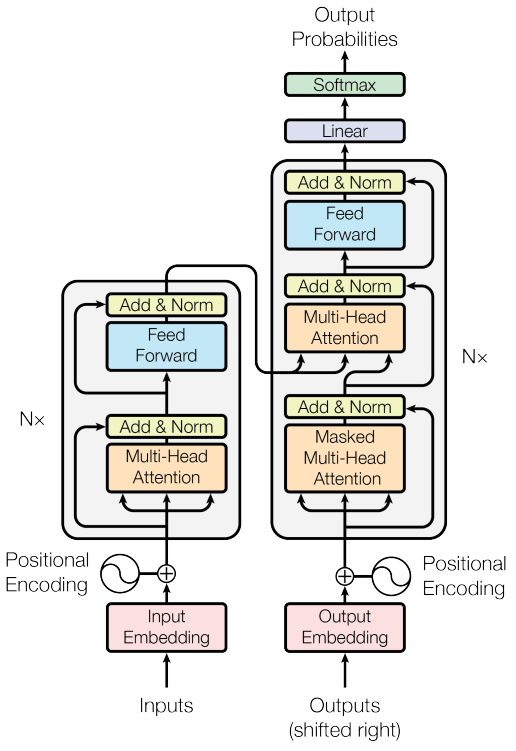
\includegraphics[width=0.5\textwidth]{Bilder/Transformer-Modell}
   \caption{Transformer-Architektur, übernommen aus Vaswani et al. (2017) \cite{vaswani2017attention}}
    \label{fig:transformer}
\end{figure}


Was diese Modelle leistungsfähig macht, ist ihr Pretraining auf gigantischen Textkorpora, bestehend aus Milliarden von Wörtern, kombiniert mit der Fähigkeit zum „Few-Shot Learning“ und „Prompt Engineering“ (vgl. \textcite{brown}) . Damit können sie eine Vielzahl sprachlicher Aufgaben bearbeiten von Übersetzungen und Zusammenfassungen über Konversationsführung bis hin zur inhaltlichen Bewertung offener Antworten. In Lernsystemen kommt diesem Aspekt besondere Bedeutung zu: Durch den Einsatz generativer KI können Freitextantworten semantisch interpretiert und kontextbezogen bewertet werden; ein klarer Fortschritt gegenüber statischen Regelwerken.

Die Bedeutung generativer KI-Technologien liegt daher nicht nur in ihrer technischen Raffinesse, sondern vor allem in ihrem disruptiven Potenzial: Sie ermöglichen eine neue Qualität der Mensch-Maschine-Interaktion und bieten pädagogisch wie wirtschaftlich interessante Anwendungsmöglichkeiten. Bildungssysteme können durch solche Technologien personalisierter, adaptiver und inklusiver gestaltet werden. Insbesondere in Szenarien mit hohem Korrekturaufwand, wie bei groß angelegten Online-Kursen, versprechen generative Modelle eine signifikante Entlastung von Lehrpersonen bei gleichzeitiger Erhöhung der Bewertungsqualität.

Dennoch ist ihre Nutzung nicht unkritisch. Neben Fragen der Fairness, Transparenz und Nachvollziehbarkeit sind auch ethische und rechtliche Aspekte zu berücksichtigen, wie im Hinblick auf Datenschutz, algorithmische Verzerrungen oder Urheberrechte. Darüber hinaus stellt sich die Frage, wie solche Systeme sinnvoll in pädagogische Konzepte integriert werden können, ohne menschliche Lehrkräfte zu entwerten oder Lernende in eine passive Rolle zu drängen \parencite{luckin}.

Insgesamt lässt sich festhalten: Generative KI-Technologien sind kein Allheilmittel, aber sie bieten erhebliche Innovationspotenziale, insbesondere dann, wenn sie mit Bedacht, Transparenz und kritischem Urteilsvermögen eingesetzt werden. In diesem Projekt wird daher nicht nur auf technische Leistungsfähigkeit, sondern auch auf eine reflektierte und verantwortungsvolle Integration in die digitale Lernumgebung geachtet.

\subsection{Kostenanalyse generativer KI-Modelle zur automatisierten Antwortbewertung}
Ein zentrales Ziel dieses Projekts ist die Entwicklung eines Systems, das sowohl funktional tragfähig als auch wirtschaftlich umsetzbar ist. Die vorliegende Kostenanalyse bildet daher nicht nur die Grundlage für die Auswahl geeigneter KI-Modelle, sondern dient zugleich als Ausgangspunkt für strategische Überlegungen hinsichtlich einer potenziellen Produktivsetzung des MVP über den Kontext einer Studienarbeit hinaus. In diesem Zusammenhang werden bewusst großzügige Annahmen getroffen, um auch Szenarien mit größerer Nutzungsintensität und realwirtschaftlicher Skalierung zu berücksichtigen.

\subsubsection{Grundlagen der Token-basierten Kostenstruktur}
Die meisten aktuellen generativen KI-Systeme berechnen ihre Nutzung auf Basis sogenannter Tokens. Ein Token repräsentiert ein Texteinheit, die ein Wort, ein Satzzeichen oder einen Wortbestandteil umfassen kann. Im Englischen entsprechen 1.000 Tokens durchschnittlich 750-800 Wörtern. Für deutsche Texte liegt der Verbrauch erfahrungsgemäß höher, da längere zusammengesetzte Wörter häufiger auftreten.

Im Rahmen des Bewertungsprozesses umfasst eine typische Anfrage sowohl den Fragetext selbst als auch Kontextinformationen, Beispielantworten, Bewertungsrichtlinien und benutzerdefinierte Parameter. Zudem entsteht durch das API-Format ein technischer Overhead. Entsprechend ergibt sich für verschiedene Fragetypen ein geschätzter Tokenverbrauch zwischen 500 und 2.500 Tokens für Input sowie zwischen 10 und 1.000 Tokens für Output, abhängig von Antwortkomplexität und Rückmeldetiefe.

\begin{table}[ht]
    \centering
    \small
    \begin{tabular}{|l|l|p{7cm}|}
        \hline
        \textbf{Fragetyp} & \textbf{Geschätzte Tokens (Input)} & \textbf{Begründung} \\
        \hline
        Multiple-Choice & 500-800 & Kurze Frage, wenige Optionen, minimaler Kontext. \\
        \hline
        Ein-Wort-Antworten & 500-1.000 & Fragetext + zusätzliche Hinweise, wie Synonyme oder Groß-/Kleinschreibung zu behandeln. \\
        \hline
        Rechenfragen & 700-1.500 & Komplexere Fragestellung + Erläuterung, wie numerische Toleranzen angewendet werden. \\
        \hline
        Entweder/Oder & 500-800 & Einfacher Entscheidungsbaum, wenig Kontext erforderlich. \\
        \hline
        Schätzfragen & 1.000-1.500 & Frage + Definition der Toleranzspannen (z.B. +/-10\%) + mögliche Beispielantworten. \\
        \hline
        Lückentextfragen & 1.500-2.000 & Fragetext + mehrere mögliche richtige Antworten für Lücken + Erläuterung für Synonyme und Tippfehler. \\
        \hline
        Freitextantworten & 2.000-2.500 & Frage + umfangreicher Kontext + mögliche Zwischenschritte bei der Beurteilung. \\
        \hline
    \end{tabular}
    \caption{Geschätzter Token-Bedarf verschiedener Fragetypen mit Begründung}
    \label{tab:tokenbedarf-fragetypen}
\end{table}



Zur Modellierung einer praxisnahen Kostenstruktur wurde ein realistisches MVP-Szenario angenommen. Dieses geht von 100 Testpersonen aus, die jeweils 100 Fragen beantworten, was zu insgesamt 10.000 Anfragen führt. Diese Menge ermöglicht eine belastbare Validierung des Bewertungssystems unter realistischen Bedingungen, ohne sich auf einzelne Fragetypen zu beschränken.

Basierend auf den typischen Anforderungen der Fragetypen ergibt sich ein durchschnittlicher Tokenbedarf von:

2.000 Tokens pro Anfrage (Input)

500 Tokens pro Bewertung (Output)

Dies resultiert in einem Gesamtvolumen von 25 Millionen Tokens, aufgeteilt in 20 Millionen Input- und 5 Millionen Output-Tokens. Die Kosten werden gemäß den Preisen (Stand vgl. \textcite{openai,gemini,cohere,claude,azure,deepseek}) der gängigsten API-Anbieter berechnet, wobei der Fokus auf kostenoptimierten Modellvarianten liegt.

Die folgende Übersicht (siehe Tabelle~\ref{tab:modellkosten}) zeigt die geschätzten Gesamtkosten für das MVP bei Einsatz verschiedener Modellvarianten. Dabei wurden jeweils die günstigsten Varianten der jeweiligen Anbieter berücksichtigt.

\begin{table}[ht]
    \centering
    \small
    \begin{tabular}{|l|r|r|r|}
        \hline
        \textbf{Modell} & \textbf{Input-Kosten (USD)} & \textbf{Output-Kosten (USD)} & \textbf{Gesamtkosten (USD)} \\
        \hline
        Gemini Flash 1.5 & 1{,}50 & 1{,}50 & 3{,}00 \\
        OpenAI GPT-4o mini & 3{,}00 & 3{,}00 & 6{,}00 \\
        Cohere Command R & 3{,}00 & 3{,}00 & 6{,}00 \\
        Azure GPT-4o mini & 3{,}00 & 3{,}05 & 6{,}05 \\
        DeepSeek Chat & 5{,}40 & 5{,}50 & 10{,}90 \\
        DeepSeek Reasoner & 11{,}00 & 10{,}95 & 21{,}95 \\
        Claude 3.5 Haiku & 20{,}00 & 25{,}00 & 45{,}00 \\
        OpenAI GPT-4o & 50{,}00 & 50{,}00 & 100{,}00 \\
        Cohere Command R+ & 50{,}00 & 50{,}00 & 100{,}00 \\
        OpenAI o1 mini & 60{,}00 & 60{,}00 & 120{,}00 \\
        OpenAI o1 preview & 300{,}00 & 300{,}00 & 600{,}00 \\
        Azure o1 preview & 305{,}60 & 305{,}60 & 611{,}20 \\
        \hline
    \end{tabular}
    \caption{Vergleich der Modellkosten für Input, Output und Gesamtkosten}
    \label{tab:modellkosten}
\end{table}


Diese Übersicht verdeutlicht erhebliche Unterschiede in der Preisstruktur. Während Gemini Flash 1.5 mit einem Gesamtpreis von 3,00 USD deutlich günstiger ist, liegen leistungsstärkere Modelle wie OpenAI o1 preview oder Azure o1 preview bei über 600 USD.

Die Kostenanalyse dient in dieser frühen Phase als Orientierungsrahmen, um ökonomische Tragfähigkeit und technologische Leistungsfähigkeit gegeneinander abzuwägen. Nach einer erfolgreichen Validierung des MVP sollen weitere Untersuchungen durchgeführt werden, die sich auf qualitative Merkmale wie Bewertungsgenauigkeit, Rückmeldetiefe und Reaktionsgeschwindigkeit konzentrieren. Diese qualitativen Kriterien sind essenziell, um die langfristige Einsatzfähigkeit in professionellen Lernumgebungen zu gewährleisten.

Ein nicht zu vernachlässigender Aspekt betrifft die Skalierung und die Möglichkeit, Kosten durch intelligentes Caching zu reduzieren. Mehrere Anbieter wie Claude oder OpenAI ermöglichen die Zwischenspeicherung von Ergebnissen, wodurch identische Anfragen bei Wiederverwendung nicht erneut berechnet werden müssen. Dieser Mechanismus ist relevant bei Übungssystemen, in denen viele identische Fragen bearbeitet werden.

Zusätzlich bieten einige Modelle (wie Gemini Flash 1.5) kostenlose API-Kontingente für Testzwecke, die eine risikoarme Erprobung im Rahmen des MVP ermöglichen. Dabei gelten jedoch Begrenzungen hinsichtlich der Anzahl an Anfragen pro Tag sowie der maximalen Tokenmenge pro Minute, was bei der Integration in eine produktive Anwendung berücksichtigt werden muss.

\newpage

\subsection{Vergleich generativer KI-Modelle zur automatisierten Antwortbewertung}
Die Auswahl geeigneter KI-Modelle zur automatisierten Antwortbewertung erfolgte im vorliegenden Projekt nicht ausschließlich auf Basis technologischer Merkmale, sondern unter der zwingenden Berücksichtigung wirtschaftlicher Rahmenbedingungen. Die zuvor durchgeführte Kostenanalyse identifizierte mehrere Modelle, die im Rahmen eines begrenzten Budgets für den Aufbau eines MVP als wirtschaftlich gelten. Die nun folgende Evaluierung baut auf diesen Ergebnissen auf und untersucht ausgewählte Modelle hinsichtlich ihrer Bewertungsqualität, Effizienz und Konsistenz in konkreten Anwendungsszenarien.

Zielsetzung und Vorgehen

Ziel dieser Untersuchung ist es, generative KI-Modelle in einem kontrollierten Setting systematisch zu vergleichen. Bewertet werden unter anderem:

\begin{itemize}
  \item die Genauigkeit der Bewertung gegenüber einer erwarteten Antwort,
  \item die Flexibilität gegenüber Synonymen, Tippfehlern und alternativen Formulierungen,
  \item die Konsistenz der Ergebnisse bei mehrfacher Durchführung,
  \item sowie die Qualität des Feedbacks.
\end{itemize}

Hierzu wurde ein standardisiertes Testset entwickelt, das typische Fragetypen aus digitalen Lernumgebungen abbildet: Multiple-Choice, Ein-Wort-Antworten, Rechenaufgaben, Entweder/Oder-Fragen, Schätzfragen, Lückentextaufgaben und Freitextantworten. Jede Frage wurde in einer Prompt-Vorlage (vgl. Abb. \ref{fig:Allgemeiner Prompt}) strukturiert an die jeweilige KI übergeben, wobei die Bewertungsanweisung explizit formuliert und mit konkreten Kriterien angereichert wurde. Die getesteten Modelle waren: OpenAI GPT-4o Mini, Gemini Flash 1.5, Cohere Command R, DeepSeek Chat und Claude 3.5 Haiku.
Die in dieser Analyse verwendeten Prompts und beispielhaften Antwortbewertungen der Modelle wurden einheitlich gestaltet und sind im Anhang dokumentiert (vgl. Abschnitt \ref{anhang}). Diese stellen die Grundlage für die vergleichende Bewertung dar und erlauben eine transparente Nachvollziehbarkeit der jeweiligen Modellantworten.

\newpage

\begin{mdframed}[linewidth=1pt, backgroundcolor=gray!10, roundcorner=5pt]
\captionof{figure}{Bewertungsanweisung für die KI}
\label{fig:Allgemeiner Prompt}

Gegeben sind eine Frage, eine Antwort auf die Frage und eine erwartete richtige Antwort.\\
Bei manchen Fragetypen gibt es noch Parameter, Antwortmöglichkeiten und unterschiedliche Kriterien.\\
Bitte bewerte die gegebene Antwort mit einer Punktzahl von 0 bis 100 mithilfe der gegebenen Bewertungskriterien und gib die Antwort im gegebenen Format aus.\\
Falls nötig, gib dem User ein kurzes Feedback für die Bewertung in \textbf{"Begründung"}, da dies dem User helfen soll zu verstehen, wo seine Fehler liegen.\\
Gehe bei der Begründung nicht ausschließlich auf die Bewertungskriterien ein. Gib ein kurzes, benutzerfreundliches Feedback!

\vspace{0.5em}
\textbf{Frage:} [Hier die Testfrage einfügen]\\
\textbf{Antwort:} [Hier die Nutzerantwort einfügen]\\
\textbf{Antwort Typ:} [Hier Typ einfügen]\\
\textbf{Parameter von Typen:} [Hier Parameter einfügen]\\
\textbf{Erwartete richtige Antwort:} [Hier die korrekte Antwort einfügen]

\textbf{Bewertungskriterien:}
\begin{itemize}
  \item Ist die Antwort inhaltlich korrekt?
  \item Falls nicht ganz korrekt, welche Abweichungen sind akzeptabel?
  \item Ist die Antwort grammatikalisch richtig?
  \item Ist die Antwort vollständig?
\end{itemize}

Antwort bitte in diesem Format:
\begin{verbatim}
{
  "Punktzahl": X,
  "Begründung": "..."
}
\end{verbatim}
\end{mdframed}



\subsubsection{Ergebnisse nach Fragetyp}

1. Multiple-Choice:
Alle getesteten Modelle erkannten die korrekte Antwort mit hoher Zuverlässigkeit. In Bezug auf die Feedbackqualität zeigten insbesondere GPT-4o Mini und Claude eine ausgeprägte Erklärungskompetenz, während Gemini eher knapp, aber klar formulierte Antworten generierte.

2. Ein-Wort-Antworten:
Hier zeigten sich Unterschiede in der Toleranz gegenüber Schreibvariationen. Während GPT-4o Mini, Gemini und Cohere moderate Fehler (z.B. ``Göthe'' statt "Goethe") als fast korrekt werteten, variierte DeepSeek in der Bewertung teils erheblich. Claude war zwar konsistent, aber inhaltlich restriktiver.

3. Rechenaufgaben:
GPT-4o Mini und DeepSeek bewerteten mathematische Aufgaben nachvollziehbar, inklusive Erkennung formaler Fehler (z.B. fehlende Einheiten). Gemini hingegen zeigte Schwächen bei logischen Bewertungen und vergab teilweise unplausible Punktzahlen.

4. Entweder/Oder-Fragen:
In dieser Kategorie lieferten alle Systeme konsistente und korrekte Antworten. Unterschiede zeigten sich lediglich in der Formulierung des Feedbacks, wobei Claude und GPT-4o Mini didaktisch ansprechend formulierten.

5. Schätzfragen:
Große Differenzen zeigten sich beim Umgang mit Toleranzbereichen. GPT-4o Mini und Gemini konnten überprüfen, ob eine Antwort innerhalb eines vorgegebenen Bereichs liegt. DeepSeek und Cohere gaben bei gleicher Eingabe teils stark divergierende Punktzahlen aus. Claude bewertete hier eher konservativ und ohne exakte Berechnung.

6. Lückentextaufgaben:
Claude und GPT-4o Mini zeigten differenzierte Bewertungen, auch bei teilweise korrekten Antworten. Gemini bewertete ebenfalls gut, zeigte jedoch in Einzelfällen faktisch falsche Einschätzungen. DeepSeek reagierte empfindlich auf Reihenfolge und Tippfehler, was zu inkonsistenten Ergebnissen führte.

7. Freitextantworten:
Hier traten die stärksten Unterschiede zutage. GPT-4o Mini überzeugte mit detailliertem, konstruktivem Feedback, das sprachlich klar und didaktisch wertvoll war. Claude lieferte umfassende Einschätzungen, wenn auch weniger didaktisch. Gemini und Cohere agierten oberflächlicher, DeepSeek war stark von der Promptformulierung abhängig.

\begin{table}[h!]
\centering
\scriptsize
\renewcommand{\arraystretch}{1.2}
\begin{tabularx}{\textwidth}{>{\bfseries}l p{1.5cm} p{1.4cm} p{2cm} p{1.8cm} p{1.7cm} p{2cm}}
\toprule
Modell & Genauigkeit & Konsistenz & Feedbackqualität & Mathematische Bewertung & Toleranz-verarbeitung & Freitextanalyse \\
\midrule
GPT-4o Mini & Hoch & Hoch & Exzellent & Sehr gut & Gut & Sehr gut \\
Claude 3.5 Haiku & Hoch & Hoch & Gut & Gut & Mäßig & Gut \\
Gemini Flash 1.5 & Hoch & Stabil & Gut & Schwach & Gut & Mittel \\
Cohere Command R & Mittel & Stabil & Gut & Mittel & Schwach & Mittel \\
DeepSeek Chat & Mittel & Variabel & Mäßig & Gut & Inkonsequent & Mäßig \\
\bottomrule
\end{tabularx}
\caption{Vergleich der Modelleigenschaften verschiedener generativer KI-Systeme}
\end{table}

Basierend auf diesen Ergebnissen empfiehlt sich GPT-4o Mini als Standardmodell für die automatisierte Bewertung von Antworten. Es bietet die beste Kombination aus Genauigkeit, Flexibilität, Feedbackqualität und Reproduzierbarkeit. Claude eignet sich als sinnvolle Alternative, insbesondere wenn der Fokus auf verständlicher Erklärung liegt. Gemini kann zur schnellen, kostengünstigen Erstbewertung herangezogen werden, ist jedoch für komplexe Aufgaben begrenzt geeignet. Cohere und DeepSeek sollten gezielt nur in Szenarien mit niedrigem Feedbackanspruch oder als Zweitinstanz eingesetzt werden.

\subsubsection{Fazit}

Die Evaluation zeigt, dass sich die Auswahl eines KI-Modells nicht allein am Preis orientieren darf. Bei offenen Fragetypen, in denen Kontextverständnis und sprachliche Nuancierung eine zentrale Rolle spielen, bietet GPT-4o Mini derzeit die leistungsstärkste und didaktisch wertvollste Lösung für automatisierte Lernbewertungen.

\section{Vergleich von KI und klassischen Algorithmen zum Bewertung}
Die Bewertung von Antworten ist ein zentrales Element in der Konzeption und Durchführung digitaler Lernumgebungen. Sie bestimmt nicht nur den Lernerfolg auf formaler Ebene, sondern beeinflusst maßgeblich auch die Wahrnehmung von Fairness, Transparenz und pädagogischer Qualität. Vor dem Hintergrund wachsender technischer Möglichkeiten stellt sich die Frage, welche Ansätze sich für die automatisierte Bewertung am besten eignen, klassische, regelbasierte Algorithmen oder moderne Verfahren auf Basis generativer Künstlicher Intelligenz (GenAI).

Ziel dieses Kapitels ist es, beide Ansätze systematisch gegenüberzustellen. Dabei erfolgt die Analyse entlang der verschiedenen Fragetypen, die typischerweise in digitalen Lernsystemen auftreten: Multiple-Choice-, Ein-Wort-, Rechen-, Schätz-, Lückentext- und Freitextfragen. Für jeden Fragetyp wird untersucht, inwieweit klassische Algorithmen eine präzise und faire Bewertung ermöglichen oder ob die Flexibilität und Kontextsensitivität generativer KI einen signifikanten Vorteil bietet. Die Analyse erfolgt entlang zentraler Bewertungskriterien: Genauigkeit, Effizienz, Kosten sowie Anpassungsfähigkeit an benutzerdefinierte Bewertungseinstellungen wie Fehlertoleranz, Groß-/Kleinschreibung oder Synonymakzeptanz.

Durch diesen Vergleich soll ein differenziertes Verständnis darüber gewonnen werden, für welche Fragetypen klassische Algorithmen nach wie vor die bevorzugte Lösung darstellen und in welchen Szenarien der Einsatz generativer KI-Technologien tatsächlich einen Mehrwert bietet, sowohl aus technischer als auch aus pädagogischer Perspektive.

\subsection{Bewertung von Multiple-Choice- und Entweder/Oder-Fragen}
Im Rahmen der Bewertung von Multiple-Choice- und Entweder/Oder-Fragen zeigen klassische algorithmische Verfahren ihre besondere Stärke. Diese Fragetypen zeichnen sich dadurch aus, dass sie auf einer klar definierten, vorher festgelegten Menge an Antwortoptionen basieren. Daraus ergibt sich ein deterministisches Bewertungsschema, das sich mit hoher Effizienz und Genauigkeit implementieren lässt. Klassische Algorithmen wie der vergleichsbasierte Abgleich sowie gewichtete Punktesysteme eignen sich hier hervorragend. Sie bieten transparente, reproduzierbare Ergebnisse und lassen sich leicht an benutzerdefinierte Einstellungen anpassen.

Beim vergleichsbasierten Abgleich wird die vom Nutzer gewählte Antwort direkt mit der als korrekt gespeicherten Option verglichen. Dieser Vergleich kann in Form eines Set-Vergleichs, einer Sortierung oder einer einfachen Lookup-Operation realisiert werden. Die Bewertung erfolgt binär (richtig/falsch) oder durch Zuweisung gewichteter Punkte. Letzteres erlaubt differenziertere Bewertungen, wie bei teilkorrekten Mehrfachantworten oder bei der Berücksichtigung von Distraktoren (\cite{RoedigerMarsh2005}).

Gewichtete Punktesysteme erweitern diesen Ansatz, indem sie jeder Antwortoption einen spezifischen Wert zuweisen (vgl. \ref{fig:Allgemeiner Prompt}). Dadurch kann eine feinere Unterscheidung zwischen vollständig richtigen, teilweise richtigen und klar falschen Antworten getroffen werden. Ein Beispiel: In einer Frage mit vier Auswahlmöglichkeiten erhalten die zwei richtigen Antworten jeweils 0,5 Punkte, während die falschen Optionen mit 0 Punkten gewichtet sind. Wählt ein Nutzer nur eine korrekte Antwort, erhält er anteilig 0,5 Punkte. Diese Systeme können optional durch negative Gewichtungen ergänzt werden, um beispielsweise erratene oder bewusst irreführende Antworten abzuwerten.

\begin{figure}[H]
    \centering
    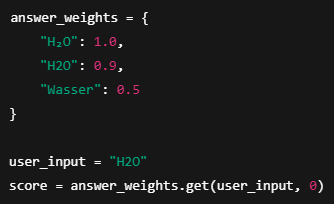
\includegraphics[width=0.5\textwidth]{Bilder/GewichtetePunkte}
   \caption{Beispiel einer Implementierung eines Gewichteten Punktesystems}
    \label{fig:transformer}
\end{figure}

Die Genauigkeit dieser klassischen Verfahren ist bei strukturierten Fragetypen wie Multiple-Choice oder Entweder/Oder nahezu optimal, da die Bewertungsregeln eindeutig sind und keine semantische Interpretation notwendig ist. Gleichzeitig sind diese Algorithmen sehr effizient: Sie benötigen nur geringe Rechenleistung, liefern sofortige Ergebnisse und lassen sich problemlos in Echtzeitsysteme integrieren. Auch aus Kostensicht sind sie klar im Vorteil: Ihre Implementierung ist einfach, es entstehen keine API-Nutzungskosten und sie benötigen keine externen Ressourcen.

Demgegenüber zeigt sich, dass der Einsatz generativer KI bei diesen Fragetypen in den meisten Fällen nicht notwendig ist und sogar zu unnötiger Komplexität führen kann. Zwar wäre eine KI in der Lage, auch Multiple-Choice-Fragen zu bewerten, sie würde dabei jedoch Rechenressourcen verbrauchen, deren Nutzen in keinem Verhältnis zum Ergebnis steht. Zudem besteht bei generativen Modellen die Gefahr von Inkonsistenzen, zum Beispiel bei identischen Antworten in leicht unterschiedlichen Kontexten. Gerade bei Bewertungsaufgaben, die maximale Reproduzierbarkeit erfordern, ist diese Eigenschaft kritisch.

In der Gesamtbetrachtung sind klassische Bewertungsalgorithmen für Multiple-Choice- und Entweder/Oder-Fragen die bevorzugte Lösung. Sie sind effizient zu implementieren, performant, kosteneffizient und hochgradig zuverlässig. Ihre Erweiterbarkeit um Benutzeroptionen wie Groß-/Kleinschreibung oder Teilpunktvergabe macht sie auch für anspruchsvollere Anwendungsfälle geeignet. Der Einsatz von generativer KI sollte auf jene Fragetypen beschränkt bleiben, bei denen kontextuelle Deutungen, sprachliche Varianten und semantische Tiefenanalyse erforderlich sind.

\subsubsection{Effizienznachweis vergleichsbasierter Bewertungsalgorithmen}

Die Bewertung strukturierter Fragetypen wie Multiple-Choice- und Entweder/Oder-Aufgaben lässt sich durch klassische deterministische Verfahren effizient realisieren. Dies liegt an der klar definierten Struktur der Antwortoptionen sowie an der Möglichkeit, deren Bewertung auf einfache Mengenoperationen oder gewichtete Summen zurückzuführen. Im Folgenden wird die geringe Rechenkomplexität dieser Verfahren formal dargelegt.

\subsubsection{Vergleichsbasierter Abgleich}

Beim binären Vergleich einer gegebenen Antwort \( a \in \mathcal{A} \) mit der korrekten Antwortmenge \( \mathcal{R} \subseteq \mathcal{A} \) erfolgt die Bewertung durch die logische Abfrage:

\[
\text{Score}(a) = 
\begin{cases}
1, & \text{wenn } a \in \mathcal{R} \\
0, & \text{sonst}
\end{cases}
\]

Für \( n = |\mathcal{R}| \) ergibt sich bei Nutzung effizienter Datenstrukturen wie Hash-Sets eine erwartete Laufzeit von \( \mathcal{O}(1) \). Im ungünstigeren Fall eines linearen Vergleichs (z.~B. bei Arrays oder Listen) beträgt die Laufzeit \( \mathcal{O}(n) \), wobei \( n \) typischerweise sehr klein ist (z.~B. \( n \leq 5 \)).

\subsubsection{Gewichtetes Punktesystem}

Erweitert man das Bewertungsschema um gewichtete Teilpunkte, so wird jeder Antwortoption \( a_i \in \mathcal{A} \) ein Gewicht \( w_i \in \mathbb{R} \) zugewiesen. Die Punktzahl des Nutzers ergibt sich dann aus der Summe der Gewichte der ausgewählten Optionen \( \mathcal{U} \subseteq \mathcal{A} \):

\[
\text{Score}(\mathcal{U}) = \sum_{a_i \in \mathcal{U}} w_i
\]

Die Bewertung erfolgt durch eine einfache Iteration über \( k = |\mathcal{U}| \) Elemente. Die Laufzeit ist somit linear in der Anzahl der vom Nutzer gewählten Optionen, also \( \mathcal{O}(k) \), wobei in typischen Anwendungsfällen \( k \ll |\mathcal{A}| \).

\subsubsection{Speicher- und Laufzeitkomplexität}

Die Gesamtkomplexität klassischer Bewertungsalgorithmen lässt sich zusammenfassend wie folgt angeben:

\begin{table}[h!]
\centering
\begin{tabular}{@{}lll@{}}
\toprule
\textbf{Verfahren} & \textbf{Laufzeit} & \textbf{Speicherbedarf} \\
\midrule
Vergleich (Hash-Set)      & \( \mathcal{O}(1) \) -- \( \mathcal{O}(n) \) & \( \mathcal{O}(n) \) \\
Gewichtete Bewertung      & \( \mathcal{O}(k) \)                         & \( \mathcal{O}(n) \) \\
\bottomrule
\end{tabular}
\caption{Komplexität klassischer Bewertungsalgorithmen}
\end{table}

Dabei sind \( n \) die Anzahl möglicher Antwortoptionen und \( k \) die Anzahl tatsächlich gewählter Optionen \parencite[S. 813]{cormen}.

\subsubsection{Vergleich mit generativer KI}

Im Gegensatz dazu verwenden generative KI-Modelle wie Transformer-basierte Architekturen eine selbstaufmerksame Kontextverarbeitung, deren Komplexität im Wesentlichen quadratisch mit der Eingabelänge wächst (vgl. \textcite{vaswani2017attention}):

\[
\text{Laufzeit generativer Modelle} = \mathcal{O}(n^2 \cdot d)
\]

wobei \( n \) die Anzahl der Tokens und \( d \) die Dimension der Repräsentationen ist. Neben der höheren Rechenkomplexität benötigen solche Modelle umfangreiche GPU-Ressourcen und führen zu höheren Antwortzeiten und Betriebskosten.

\subsubsection{Schlussfolgerung}

Die hier betrachteten klassischen Bewertungsalgorithmen zeigen im Vergleich zu KI-gestützten Verfahren eine signifikant geringere Rechen- und Speicherkomplexität. Sie ermöglichen Echtzeitbewertung mit deterministischer Logik, hoher Reproduzierbarkeit und minimalem Ressourcenverbrauch. Mathematisch lässt sich ihre Effizienz durch konstante oder lineare Zeitkomplexität formal belegen. Dies macht sie zur bevorzugten Wahl für klar strukturierte Fragetypen wie Multiple-Choice und Entweder/Oder gegenüber GenAI Lösungen.
\newpage

\subsection{Bewertung von Ein-Wort-Antworten, Rechenfragen und Schätzfragen}
Ein-Wort-Antworten bilden einen Grenzbereich zwischen strukturierten und offenen Antwortformaten, da sie zwar formal knapp sind, aber inhaltlich vielfältige sprachliche Realisierungen zulassen. Klassische Bewertungsalgorithmen wie String-Matching-Verfahren sind hier nur dann zuverlässig, wenn die Antwort exakt mit der gespeicherten Lösung übereinstimmt. Bereits geringfügige Abweichungen, durch Groß- und Kleinschreibung, Tippfehler oder Synonyme, führen häufig zur Abwertung eigentlich korrekter Antworten. Durch Normalisierungen wie das Entfernen von Leerzeichen oder die Umwandlung in Kleinbuchstaben lässt sich die Widerstandsfähigkeit gegenüber formalen Abweichungen zwar verbessern, doch bleibt die grundsätzliche Einschränkung in der sprachlichen Flexibilität bestehen.

Zur Verbesserung dieser Flexibilität können Techniken wie Stemming und Lemmatisierung eingesetzt werden. Diese reduzieren Wörter auf ihre Grundformen und ermöglichen so eine verallgemeinerte, robustere Bewertung. Zusätzlich lassen sich synonyme Ausdrücke und alternative Formulierungen berücksichtigen, sofern entsprechende Sprachressourcen wie Synonymdatenbanken oder Thesauri eingebunden sind. Solche Verfahren kommen in Evaluationsmetriken wie METEOR zum Einsatz, wo sie durch die Kombination aus Lemma- und Synonymabgleich eine höhere Korrelation mit menschlichen Bewertungen erreichen \parencite[Kapitel~35.6.2]{mitkov}.

Ein Beispiel für ein System, das solche Verfahren kombiniert, ist C-rater. C-rater nutzt verschiedene linguistische Normalisierungen wie Morphologie-, Synonym- und Strukturvergleiche, um konzeptuelle Äquivalenz zwischen Schülerantworten und Modellantworten zu erkennen \parencite[vgl.][S.~389ff.]{leacock}. Das System extrahiert Prädikat-Argument-Strukturen (Tuples), normalisiert Wortformen, löst Pronomenreferenzen auf und bezieht semantisch ähnliche Begriffe über Wortähnlichkeitsmatrizen ein. Damit geht C-rater über phonetische oder stringbasierte Ähnlichkeitsverfahren hinaus und erlaubt eine kontextuell sensibilisierte Bewertung, die auf Bedeutungsentsprechung statt reinem Wortlaut basiert. Allerdings stößt C-rater bei stark variierenden oder kreativen, aber korrekten Formulierungen an Grenzen. Es ist auf vordefinierte Antwortmodelle angewiesen und erkennt nur solche Inhalte als korrekt, die zuvor explizit modelliert wurden. Dadurch kann es in offenen oder stark kontextabhängigen Antwortformaten zu sogenannten "misses" kommen, also zu fälschlich abgewerteten Antworten, obwohl das Verständnis prinzipiell vorhanden ist.

Um solchen Einschränkungen zu begegnen, bieten generative KI-Modelle eine höhere Flexibilität und Genauigkeit, vor allem bei der semantischen Bewertung unterschiedlich formulierter, aber inhaltlich äquivalenter Antworten. Darüber hinaus kann eine KI bewerten, ob ein Begriff im thematischen Kontext sinnvoll ist, und dadurch auch bei kreativeren Antworten ein differenziertes Urteil fällen. Hilfreich ist dies, wenn Nutzer eigene Formulierungen verwenden oder wenn kulturelle, sprachliche oder fachliche Unterschiede in der Ausdrucksweise bestehen. Auch die Berücksichtigung benutzerdefinierter Bewertungskriterien wie Synonymakzeptanz oder Fehlergrenzen kann in KI-Modellen flexibel integriert werden.


Bei Rechenfragen ist die Situation differenziert zu betrachten. Klassische Algorithmen können numerische Antworten sehr effizient prüfen. Insbesondere bei geschlossenen Aufgaben mit klar definiertem Ergebnis genügt ein Vergleich zwischen Nutzerantwort und Referenzwert. Allerdings endet die Leistungsfähigkeit dieser Methoden, sobald Zwischenschritte oder der Rechenweg eine Rolle spielen. Klassische Algorithmen sind nicht in der Lage, Teillösungen oder methodisch richtige, aber formal ungenaue Ansätze differenziert zu bewerten.

Zur Berücksichtigung kleiner Abweichungen, durch Rundungen, werden häufig \textit{Toleranzbereiche} eingesetzt. Diese können als absoluter Fehler, prozentualer Fehler oder in Form signifikanter Stellen definiert werden \parencite{calcme}. So kann beispielsweise ein Schülerergebnis $s_a$ als korrekt gelten, wenn es vom korrekten Wert $c_a$ nur um maximal $n$ Einheiten abweicht, also $|c_a - s_a| \leq n$. Alternativ kann ein Fehler von höchstens $n\,\%$ zulässig sein, was durch $\frac{|c_a - s_a|}{|c_a|} \leq 0{,}01 \cdot n$ ausgedrückt wird.

Zudem kann die Vergleichslogik so konfiguriert werden, dass nur die ersten $n$ signifikanten Ziffern oder Dezimalstellen mit dem exakten Wert übereinstimmen müssen. Auch periodische Dezimalzahlen, wie $0.\overline{3}$, werden korrekt erkannt und als äquivalent zu $\frac{1}{3}$ gewertet, sofern die gewählte Toleranz dies zulässt \parencite{calcme}.

Technisch ist die Umsetzung solcher Prüfmechanismen unproblematisch, insbesondere wenn die Antworten als Zahlenwerte vorliegen. Komplexer wird die Situation jedoch, wenn \textit{Rechenwege oder Zwischenschritte} Teil der Bewertung sein sollen. Klassische Bewertungsalgorithmen sind hier oftmals überfordert, da sie nur das Endergebnis prüfen und keine symbolische Herleitung nachvollziehen können.

Wie in der Dokumentation von CalcMe betont wird, lassen sich symbolische und exakte Ausdrücke (z.\,B. $\frac{1}{2}$, $\pi$, $\sqrt{2}$) intern verarbeiten, doch der Wechsel zur numerischen Bewertung kann zu Informationsverlust führen \parencite{calcme}. Um exakte Lösungen von gerundeten Werten zu unterscheiden, ist die Definition geeigneter Präzisionseinstellungen notwendig. Auch ist zu beachten, dass selbst wenn eine exakte Ganzzahl erwartet wird, ein numerisch nahegelegener Dezimalwert (z.\,B. $4.0$ statt $4$) als korrekt gewertet werden kann, sofern keine \textit{symbolische Validierung} gefordert ist \parencite{calcme}.

Insgesamt zeigt sich: Während Rechenfragen algorithmisch gut zu bewerten sind, erfordert eine differenzierte Bewertung von Lösungswegen eine aufwändigere Analyse.

Aber auch hier bietet generative KI substanzielle Vorteile: Sie kann Zwischenschritte interpretieren, den Lösungsweg analysieren und gegebenenfalls Teilpunkte vergeben, selbst wenn das Endergebnis fehlerhaft ist. Dies fördert nicht nur ein gerechteres Bewertungsergebnis, sondern gibt auch aufschlussreiches Feedback zu typischen Denkfehlern oder Missverständnissen. Damit wird die KI-basierten Bewertung ein pädagogischer Mehrwert zugeschrieben, der über die bloße Ergebnisprüfung hinausgeht.

Die Wahl des geeigneten Bewertungsverfahrens für Rechenfragen hängt maßgeblich von den Zielsetzungen der Aufgabe ab. Wenn ausschließlich das korrekte Endergebnis von Interesse ist, bei standardisierten Prüfungen oder automatisierten Tests, bieten klassische Algorithmen aufgrund ihrer geringen Komplexität und hohen Zuverlässigkeit klare Vorteile. Sie ermöglichen eine ressourcenschonende Echtzeitbewertung bei gleichzeitig hoher Reproduzierbarkeit.

Anders stellt sich die Situation dar, wenn der Lösungsweg explizit berücksichtigt oder differenziert bewertet werden soll. In solchen Fällen stoßen rein numerische Vergleichsverfahren an ihre Grenzen, da sie weder symbolische Herleitungen analysieren noch Teillösungen anerkennen können. Hier eröffnet der Einsatz generativer KI neue Möglichkeiten: Modelle wie GPT können Zwischenschritte interpretieren, methodische Korrektheit erkennen und auch bei formal fehlerhaften Endergebnissen pädagogisch sinnvolle Rückmeldungen geben.

Welche Methode im konkreten Fall vorzuziehen ist, hängt somit von verschiedenen Faktoren ab:
\begin{itemize}
  \item \textbf{Ziel der Aufgabe:} Geht es primär um das Ergebnis oder auch um den Weg dorthin?
  \item \textbf{Bewertungstiefe:} Wird eine binäre Richtig/Falsch-Wertung angestrebt oder eine differenzierte Teilpunktvergabe?
  \item \textbf{Technische Rahmenbedingungen:} Stehen ausreichend Ressourcen (Rechenleistung, Zeit, Speicher) zur Verfügung?
  \item \textbf{Pädagogischer Anspruch:} Wird Wert auf Feedback, Fehlertypenanalyse oder formative Bewertung gelegt?
\end{itemize}

Insbesondere bei großflächigen Prüfungen mit vielen Teilnehmenden kann eine hybride Herangehensweise sinnvoll sein: Während Aufgaben automatisiert durch klassische Verfahren bewertet werden, kommen KI-gestützte Analysen dort zum Einsatz, wo individuelle Lösungswege oder komplexere kognitive Leistungen im Fokus stehen. Die bewusste Kombination beider Ansätze ermöglicht eine ausgewogene Balance zwischen Effizienz und pädagogischer Qualität.

Wie bei Rechenfragen ist auch bei Schätzfragen die Angemessenheit von Toleranzbereichen zentral. Während klassische Algorithmen durch definierte Toleranzbereiche (z.B. ±10\% vom korrekten Wert) nachvollziehbare Bewertungen ermöglichen, stoßen sie an ihre Grenzen, wenn Antworten im Kontext beurteilt werden sollen. Eine Nutzerantwort mag zwar numerisch außerhalb des Toleranzintervalls liegen, kann aber dennoch nachvollziehbar und fachlich plausibel sein. Klassische Verfahren erkennen diesen Unterschied nicht.

Generative KI hingegen kann nicht nur prüfen, ob eine Antwort innerhalb eines festgelegten Bereichs liegt, sondern auch deren argumentative Herleitung bewerten. Wenn der Rechenweg oder die Annahmen hinter einer Schätzung angegeben werden, ist die KI in der Lage, diese zu analysieren und eine differenzierte Bewertung abzugeben. Insbesondere bei interdisziplinären oder realitätsnahen Aufgabenstellungen ist dies ein großer Vorteil, da die Antwort nicht nur als Zahl, sondern im Kontext einer Problemstellung interpretiert wird.

Zusammenfassend lässt sich sagen, dass klassische Algorithmen bei Ein-Wort-, Rechen- und Schätzfragen vor allem dann geeignet sind, wenn die Bewertungsregeln einfach und deterministisch sind. Sobald jedoch inhaltliche Tiefe, kontextuelle Einbettung oder methodische Nachvollziehbarkeit gefordert sind, bietet die generative KI mehr Flexibilität und pädagogische Qualität. Der gezielte Einsatz beider Ansätze, je nach Fragetyp und Zielsetzung, stellt daher den vielversprechendsten Weg dar, um automatisierte Lernbewertungen effektiv und gerecht zu gestalten.

\subsubsection{Effizienznachweis numerikbasierter Bewertungsalgorithmen}

Im Gegensatz zu offenen Textantworten lassen sich numerische Antworten mithilfe klassischer Bewertungsalgorithmen äußerst effizient verarbeiten. Die zugrunde liegende Logik basiert auf arithmetischen Vergleichen zwischen einem Referenzwert \( c_a \) und einer Nutzerantwort \( s_a \), ergänzt durch definierbare Toleranzbereiche. Diese Bewertungsformen sind mathematisch exakt beschreibbar und benötigen lediglich elementare Rechenoperationen, was sie performant und ressourcenschonend macht.

Eine typische Validierungsregel in Form eines absoluten Fehlers lautet:

\[
|c_a - s_a| \leq \varepsilon
\]

mit \(\varepsilon\) als frei wählbarem Toleranzparameter. Die Prüfung erfolgt in konstanter Zeit \( \mathcal{O}(1) \), da lediglich eine Subtraktion, Betragsbildung und Vergleichsoperation notwendig ist. Entsprechendes gilt für relative Fehler:

\[
\frac{|c_a - s_a|}{|c_a|} \leq \delta
\]

Diese Verfahren sind insbesondere bei geschlossenen Rechenfragen mit exakt definierter Zielgröße effektiv einsetzbar. Systeme wie \textit{CalcMe} unterstützen darüber hinaus weitere numerische Vergleichsmethoden wie die Überprüfung signifikanter Stellen, Dezimalstellen oder die Erkennung periodischer Dezimaldarstellungen \parencite{calcme}. Auch diese Methoden basieren auf festen mathematischen Regeln und lassen sich mit deterministischen Algorithmen effizient umsetzen.

Die allgemeine Laufzeit solcher Bewertungsalgorithmen beträgt:

\[
\text{Laufzeit} = \mathcal{O}(1)
\]

sowohl für absolute als auch prozentuale Fehlergrenzen. Bei signifikanter Stellenzahl oder Dezimalstellenvergleich kann ein zusätzlicher Trunkierungs- oder Rundungsschritt notwendig sein, der jedoch in konstantem oder bestenfalls logarithmischem Aufwand realisierbar ist, abhängig von der Repräsentation der Zahlen.

\begin{table}[h!]
\centering
\begin{tabular}{@{}lll@{}}
\toprule
\textbf{Verfahren} & \textbf{Laufzeit} & \textbf{Speicherbedarf} \\
\midrule
Absoluter Fehlervergleich & \( \mathcal{O}(1) \) & \( \mathcal{O}(1) \) \\
Prozentualer Fehlervergleich & \( \mathcal{O}(1) \) & \( \mathcal{O}(1) \) \\
Signifikante Stellen & \( \mathcal{O}(1) \) - \( \mathcal{O}(\log n) \) & \( \mathcal{O}(1) \) \\
\bottomrule
\end{tabular}
\caption{Komplexität numerischer Bewertungsalgorithmen nach Toleranztyp}
\end{table}

Die Bewertung numerischer Aufgaben erfolgt somit mit minimalem Ressourcenverbrauch, hoher Reproduzierbarkeit und in Echtzeit. Im didaktischen Kontext ist diese Effizienz von Bedeutung, da so auch großskalige Prüfungen ohne signifikanten Rechenaufwand automatisiert durchgeführt werden können. Die Implementierung solcher Systeme ist im Vergleich zur semantischen Analyse einfacher, robust gegenüber Skalierung und auch kostenseitig klar im Vorteil.




\subsection{Bewertung von Lückentexten und Freitexten}
Lückentext- und Freitextfragen gehören zu den anspruchsvollsten Fragetypen in digitalen Lernumgebungen, insbesondere im Hinblick auf die automatisierte Bewertung. Beide Formate verlangen vom System die Fähigkeit, Sprache nicht nur formell, sondern auch inhaltlich und kontextuell zu verstehen. Dies stellt klassische, regelbasierte Algorithmen vor erhebliche Herausforderungen, während generative KI-Modelle hier ihre Stärken ausspielen können.

Lückentextfragen weisen eine formale Struktur auf, in der definierte Leerstellen durch die Lernenden ausgefüllt werden müssen. Die Bewertung klassischer Systeme basiert häufig auf direkter Wortübereinstimmung (String-Matching) pro Lücke. Dies ist effizient und deterministisch, stößt jedoch schnell an Grenzen, sobald alternative, aber gleichwertige Begriffe (z.B. Synonyme) oder kleinere orthografische Abweichungen vorkommen. Bereits unterschiedliche Groß-/Kleinschreibung, Varianten wie „CO₂“ vs. „Kohlendioxid“ oder fehlerhafte Interpunktion können zur Abwertung führen, obwohl die semantische Bedeutung der Antwort korrekt ist.

Der Einsatz klassischer Algorithmen bei Lückentexten kann durch optionale Normalisierungen wie Case-Folding (lower()) und Whitespace-Trimming verbessert werden. Auch Fehlertoleranzen lassen sich über Levenshtein-Distanz implementieren \parencite{jurafsky}. Doch diese Verfahren stoßen dort an ihre Grenzen, wo semantische Äquivalenz statt formaler Übereinstimmung gefordert ist. Dies betrifft insbesondere Fragen mit mehreren möglichen korrekten Antworten oder solche, die fachspezifische Begrifflichkeiten verlangen.

Generative KI hingegen kann Antworten inhaltlich und kontextsensitiv analysieren. Sie erkennt Synonyme, verarbeitet Tippfehler tolerant, akzeptiert alternative Bezeichnungen und kann teilweise richtige Antworten differenziert bewerten. So können auch Lernende, die eine richtige, aber anders formulierte Lösung wählen, fair beurteilt werden. Zudem erlaubt die KI differenziertes Feedback pro Lücke: Anstelle einer Nullbewertung bei Abweichung bietet sie erklärende Rückmeldungen, die den Lernfortschritt fördern.

Die Bewertung von Freitextantworten stellt eine der größten Herausforderungen in der automatisierten Lernstandsanalyse dar. Ausdrucksweise, Satzbau, Argumentationsstruktur und thematische Kohärenz variieren stark zwischen den Lernenden. Aspekte, die sich mit klassischen, oberflächlichen Algorithmen nur begrenzt abbilden lassen.

Ein häufig verwendetes Verfahren zur automatisierten Bewertung von Lernendenantworten ist das sogenannte Keyword-Matching. Dabei wird überprüft, ob bestimmte zuvor definierte Schlüsselbegriffe oder Phrasen, die in einer Musterlösung enthalten sind, auch in der Antwort der lernenden Person vorkommen. Diese Methode ist technisch vergleichsweise einfach umzusetzen und ermöglicht eine schnelle Bewertung großer Textmengen. Allerdings weist das Verfahren erhebliche inhaltliche Schwächen auf.

Insbesondere kann es zu sogenannten false negatives kommen, wenn eine inhaltlich korrekte Antwort gegeben wird, die jedoch semantisch äquivalente Formulierungen anstelle der exakt erwarteten Schlüsselbegriffe verwendet. Ebenso kann es zu false positives führen, wenn inhaltlich falsche oder irrelevante Aussagen lediglich deshalb als korrekt gewertet werden, weil sie die gesuchten Begriffe enthalten. Diese Probleme resultieren daraus, dass Keyword-Matching lediglich auf der Oberflächenstruktur des Textes operiert und die Bedeutung sprachlicher Äußerungen nicht direkt, sondern nur über das Vorhandensein spezifischer Lexeme erschließen kann \parencite{burrows}.

Ein Beispiel hierfür wäre die Bewertung der folgenden drei Sätze:
\begin{verbatim}
(1) „The hare beats the tortoise.“
(2) „The tortoise beats the hare.“
(3) „The tortoise was beaten by the hare.“
\end{verbatim}
Während ein einfaches bag-of-words-Modell (wie beim Keyword-Matching) (1) und (2) als gleichwertig einstufen könnte, obwohl sie gegenteilige Bedeutungen haben, erkennt ein semantisch fundierteres Modell wie das Lexical-Resource-Scoring (LRS), dass (1) und (3) inhaltlich äquivalent sind, da beide denselben Sachverhalt ausdrücken, nur in unterschiedlicher Formulierung \parencite[S. 74]{burrows}.

Ein differenzierteres Verfahren ist das N-gram-Matching, das Übereinstimmungen auf Ebene von Wortgruppen untersucht, typischerweise 2- bis 5-Wort-Sequenzen. Diese Methode erlaubt eine granularere Analyse von Textmustern \parencite{jurafsky}, bleibt aber dennoch auf die syntaktische Oberfläche beschränkt. Sie prüft lediglich, ob bestimmte Wortfolgen auftreten, ohne deren Bedeutung oder semantische Funktion im Textkontext zu erfassen. In der computational linguistics community wird N-gram-basierten Verfahren deshalb eine begrenzte Ausdruckskraft im Hinblick auf tieferes Sprachverständnis zugeschrieben \parencite{mitkov}.

Um diese Limitierungen zu überwinden, können generative KI-Modelle zum Einsatz kommen. Diese sind in der Lage, Antworten auf semantischer Ebene zu analysieren, erkennen logische Zusammenhänge, fachliche Begriffe und stilistische Feinheiten. Sie berücksichtigen nicht nur, ob ein Konzept erwähnt wird, sondern auch, ob es korrekt dargestellt oder argumentativ eingebettet ist. Außerdem erlauben sie eine flexible Anpassung der Bewertungsmaßstäbe, z.B. über Prompt-Design, das festlegt, ob einfache Sprache oder eine präzise wissenschaftliche Ausdrucksweise erwartet wird.

Damit eröffnen sich neue Wege für eine faire, inhaltsbasierte Bewertung, die über formale Wortübereinstimmung hinausgeht, eine entscheidende Voraussetzung, um Freitextfragen sinnvoll in digitalen Lernumgebungen einzusetzen.

\subsubsection{Effizienznachweis für Lückentext- und Freitextbewertung}

Die automatisierte Bewertung von Lückentext- und Freitextfragen stellt auch aus Effizienzsicht eine besondere Herausforderung dar. Während klassische Algorithmen bei Lückentexten zumindest teilweise strukturierte Ansätze verfolgen können, sind Freitextantworten durch ihre inhärente Offenheit und sprachliche Variabilität wesentlich rechenintensiver, insbesondere bei Einsatz generativer KI-Modelle.\\



\textbf{Klassische Verfahren für Lückentexte}  

Bei Lückentexten lassen sich klassische Bewertungsalgorithmen auf jede Lücke einzeln anwenden. Die Bewertung erfolgt über exaktes String-Matching oder Varianten davon (z.\,B. Case-Folding, Trimming, Levenshtein-Distanz). Die durchschnittliche Laufzeit ergibt sich für $k$ Lücken wie folgt:

\[
\text{Laufzeit}_{\text{klassisch}} = \sum_{i=1}^{k} \mathcal{O}(f_i)
\]

wobei $f_i$ die Komplexität der Vergleichsfunktion pro Lücke bezeichnet.  
Bei einem Stringvergleich beträgt diese konstant \(\mathcal{O}(1)\); bei Einsatz der Levenshtein-Distanz steigt sie typischerweise auf \(\mathcal{O}(m \cdot n)\), wobei \(m\) und \(n\) die Längen der zu vergleichenden Zeichenketten sind \parencite[S. 985]{cormen}.\\

\textbf{Klassische Verfahren für Freitextantworten} 

Für Freitextantworten sind klassische Algorithmen wie Keyword- oder N-Gram-Matching vergleichsweise schnell, z.\,B. mit einer Laufzeit von

\[
\mathcal{O}(n \cdot m)
\]

für \(n\) Wörter im Text und \(m\) definierte Schlüsselbegriffe. Allerdings sind diese Verfahren in ihrer semantischen Tiefe begrenzt \parencite{navarro, jurafsky}.\\

\textbf{Generative KI bei Lücken- und Freitexten}  

Die Bewertung durch generative KI-Modelle (z.\,B. GPT) erfolgt durch semantische Analyse ganzer Textpassagen. Diese Modelle verarbeiten Texte in Tokenform mithilfe von Self-Attention-Mechanismen. Die Komplexität steigt quadratisch mit der Eingabelänge:

\[
\text{Laufzeit}_{\text{KI}} = \mathcal{O}(n^2 \cdot d)
\]

Dabei ist \(n\) die Anzahl der Tokens und \(d\) die Dimension der Repräsentationsvektoren. Bei längeren Antworten (z.\,B. 200-500 Tokens) führt dies zu höheren Antwortzeiten und Rechenlasten.\\

\newpage
\textbf{Vergleich der Verfahren}  
\begin{table}[h!]
\centering
\begin{tabular}{@{}lll@{}}
\toprule
\textbf{Verfahren} & \textbf{Laufzeit} & \textbf{Eignung für Echtzeit} \\
\midrule
Lückentext (String-Vergleich) & \( \mathcal{O}(k) \) & Hoch \\
Lückentext (Levenshtein) & \( \mathcal{O}(k \cdot m \cdot n) \) & Mittel \\
Freitext (Keyword/N-Gram) & \( \mathcal{O}(n \cdot m) \) & Mittel \\
Lücken-/Freitext (KI-basiert) & \( \mathcal{O}(n^2 \cdot d) \) & Gering bis Mittel \\
\bottomrule
\end{tabular}
\caption{Vergleich der Bewertungsverfahren bei Lücken- und Freitextaufgaben}
\end{table}\\

\textbf{Fazit}

Während klassische Verfahren bei Lückentexten in Bezug auf Rechenaufwand effizient bleiben, benötigen sie aufwändige Erweiterungen für semantische Robustheit. Freitextbewertungen hingegen sind durch klassische Algorithmen nur begrenzt sinnvoll umsetzbar. Generative KI liefert hier bessere pädagogische Ergebnisse, ist jedoch wesentlich rechenintensiver. Der Einsatz von GenAI empfiehlt sich daher insbesondere bei qualitativ hochwertigen Bewertungen, sofern ausreichende Ressourcen vorhanden sind.

\newpage

\section{Technologien und Architektur}
Die technische Umsetzung des Projekts basiert auf einem modernen Fullstack-Ansatz, der eine klare Trennung zwischen Frontend, Backend, Datenhaltung und API-Kommunikation vorsieht. Die Architektur des entwickelten Systems folgt einem serviceorientierten und modularen Design, das sich durch eine klare Trennung von Präsentation, Geschäftslogik, Datenhaltung und externen Schnittstellen auszeichnet. Im Folgenden werden die eingesetzten Technologien systematisch beschrieben.
\subsection{Frontend}
Die Benutzeroberfläche wurde mit Angular, einem auf TypeScript basierenden Frontend-Framework von Google, realisiert. Angular ist geeignet für die Entwicklung von Single-Page Applications (SPA), bei denen der Inhalt dynamisch aktualisiert wird, ohne die gesamte Seite neu zu laden. Die Vorteile von Angular liegen in seiner klaren Struktur, der engen Verzahnung mit TypeScript sowie der komponentenbasierten Architektur. Die Wahl fiel bewusst auf Angular, da es eine solide Basis für strukturierte Projekte mit komplexer Formularlogik bietet. Der Einsatz von Reactive Forms ermöglicht eine präzise Validierung und Zustandsverwaltung der Benutzereingaben.


\begin{itemize}
    \item \textbf{TypeScript} als Basissprache für alle Komponenten: Durch statische Typisierung erhöht sich die Fehlervermeidung bereits zur Entwicklungszeit.
    
    \item \textbf{Reactive Forms} für die Verwaltung komplexer Formulare und Zustände: Dieses Formularmodell ermöglicht es, Benutzereingaben programmatisch zu validieren und dynamisch zu reagieren.
    
    \item \textbf{Routing mit \texttt{RouterModule}} zur Navigation zwischen Komponenten wie \textit{Login}, \textit{Fragenverwaltung}, \textit{Prüfungsbearbeitung} und \textit{Ergebnisse}.
    
    \item \textbf{SCSS (Sassy CSS)} als CSS-Präprozessor: Erlaubt die Nutzung von Variablen, Verschachtelungen und Mixins, was zu einer besseren Strukturierung und Wiederverwendbarkeit des Stylesheets führt.
    
    \item \textbf{Internationalisierung mit \texttt{ngx-translate}}: Die App ist mehrsprachig konzipiert und kann problemlos um weitere Sprachpakete erweitert werden.
    
    \item \textbf{HttpClient}: Für den asynchronen Datenaustausch mit dem Backend über RESTful APIs.
\end{itemize}

Das Frontend der Anwendung ist responsiv gestaltet und stellt eine benutzerfreundliche Oberfläche bereit. Als Basissprache kommt TypeScript zum Einsatz, was durch statische Typisierung eine frühzeitige Fehlervermeidung während der Entwicklung ermöglicht. Für die Verwaltung komplexer Formulare und Zustände wird das \textit{Reactive Forms}-Modell verwendet. Dieses erlaubt es, Benutzereingaben programmatisch zu validieren und dynamisch auf Änderungen zu reagieren. Die Navigation innerhalb der Anwendung erfolgt über das \textit{RouterModule}, welches den Wechsel zwischen Komponenten wie Login, Fragenverwaltung, Prüfungsbearbeitung und Ergebnisanzeige unterstützt.

Zur Strukturierung und besseren Wartbarkeit der Stylesheets wird der CSS-Präprozessor SCSS verwendet. Dieser ermöglicht unter anderem die Nutzung von Variablen, Verschachtelungen und Mixins. Die Internationalisierung der Anwendung erfolgt mit Hilfe von \texttt{ngx-} \texttt{translate}, wodurch eine mehrsprachige Nutzung realisiert und einfach erweitert werden kann. Der Datenaustausch mit dem Backend erfolgt asynchron über RESTful APIs mittels \textit{HttpClient}.

Das Frontend der Anwendung ist responsiv gestaltet und stellt eine benutzerfreundliche Oberfläche zur Verfügung. Entwickelt wurde es mit TypeScript als Basissprache, wodurch durch statische Typisierung bereits zur Entwicklungszeit eine höhere Fehlervermeidung gewährleistet wird. Die Verwaltung komplexer Formulare erfolgt mithilfe des \textit{Reactive Forms}-Modells, das eine programmgesteuerte Validierung von Eingaben sowie eine dynamische Reaktion auf Zustandsänderungen ermöglicht. Die Navigation zwischen den einzelnen Komponenten, z.B. Login, Fragenverwaltung, Prüfungsbearbeitung oder Ergebnisanzeige, wird durch das \textit{RouterModule} realisiert.

Für die Gestaltung des Layouts kommt der CSS-Präprozessor SCSS zum Einsatz, der unter anderem die Nutzung von Variablen, Verschachtelungen und Mixins erlaubt und somit zu einer besseren Strukturierung und Wiederverwendbarkeit des Stylesheets beiträgt. Die Anwendung ist mehrsprachig konzipiert und nutzt zur Internationalisierung die Bibliothek \texttt{ngx-translate}, wodurch eine Erweiterung um zusätzliche Sprachpakete möglich ist. Der Datenaustausch mit dem Backend erfolgt über den \textit{HttpClient} asynchron über RESTful APIs.

Funktional bietet das Frontend unter anderem ein Benutzerprofil, das Zugriff auf persönliche Einstellungen sowie die Ergebnisse abgeschlossener Prüfungen ermöglicht. Nutzer können eigenständig Fragen erstellen, bearbeiten und löschen. Diese Fragen können im Anschluss Prüfungen zugewiesen werden, wobei sich die Prüfungen zusätzlich um ein Zeitlimit konfigurieren lassen. Während der Durchführung einer Prüfung stehen Funktionen wie eine Fortschrittsanzeige, die Navigation zwischen einzelnen Fragen sowie ein Echtzeit-Timer zur Verfügung. Nach Abschluss wird die Abgabe automatisiert an eine externe Schnittstelle gesendet, die auf der ChatGPT-API basiert. Diese übernimmt die KI-gestützte Korrektur der Prüfung und liefert eine entsprechende Bewertung samt Feedback zurück.

\subsection{Backend}

Das serverseitige System wurde mit ASP.NET Core 7 entwickelt, einem modernen, plattformunabhängigen Webframework von Microsoft, das sich durch hohe Performance, Skalierbarkeit und Flexibilität auszeichnet. Das Backend folgt dem Prinzip einer klar strukturierten Schichtenarchitektur. In der obersten Ebene befindet sich die Controller-Schicht, die für das Routing und die Entgegennahme von HTTP-Anfragen verantwortlich ist. Sie übernimmt außerdem die Autorisierung und delegiert fachliche Aufgaben an die zugrunde liegende Service-Schicht. Diese Schicht implementiert die Geschäftslogik der Anwendung, die Validierung von Prüfungen, das Anlegen von Versuchen oder die Übergabe von Abgaben an das Bewertungssystem.

Die Repository-Schicht bildet die unterste Ebene der Architektur und ist für den Datenzugriff zuständig. Sie nutzt das Object-Relational-Mapping-Framework Entity Framework Core (EF Core), um eine effiziente und typensichere Interaktion mit der Datenbank zu gewährleisten.

Zur weiteren Unterstützung einer sauberen Softwarearchitektur kommen zusätzliche Konzepte und Technologien zum Einsatz. Die native Unterstützung von Dependency Injection (DI) in ASP.NET Core ermöglicht eine klare Trennung zwischen Implementierung und Abhängigkeiten durch die Verwendung von Interfaces. Sämtliche Datenzugriffe und API-Aufrufe sind asynchron realisiert, wodurch eine nicht-blockierende Verarbeitung durch das \texttt{async/await}-Paradigma sichergestellt wird. Die Authentifizierung erfolgt mittels JSON Web Tokens (JWT), die nach dem Login generiert, clientseitig gespeichert und bei jeder weiteren Anfrage im HTTP-Header mitgesendet werden.

Die bereitgestellte REST-API umfasst Endpunkte für die Benutzerregistrierung und -anmeldung, die Verwaltung von Fragen und Prüfungen, das Starten und Abschließen von Prüfungsversuchen sowie die Rückgabe von Ergebnissen, einschließlich einer automatisierten Bewertung durch die Integration eines generativen KI-Moduls auf Basis von ChatGPT.


\subsection{Accountsicherheit und Authentifizierung}

Die Benutzerauthentifizierung im System erfolgt auf Basis eines rollenunabhängigen, tokenbasierten Sicherheitskonzepts, das sowohl Zugriffsschutz als auch Wiederanmeldemechanismen umfasst. Für den Login wird ein klassisches E-Mail/Passwort-Verfahren eingesetzt, bei dem alle Passwörter serverseitig mit dem BCrypt-Hashing-Algorithmus gesichert werden. Dies gewährleistet eine starke Einwegverschlüsselung und schützt vor dem Auslesen sensibler Zugangsdaten selbst im Falle eines Datenlecks.

Nach erfolgreicher Anmeldung wird ein zeitlich begrenzt gültiger \textit{Access Token} in Form eines JSON Web Token (JWT) erzeugt. Dieser enthält standardisierte Claims wie \texttt{sub} (Benutzer-ID), \texttt{name} (Benutzername) und \texttt{exp} (Ablaufzeitpunkt). Der Token wird mit dem Algorithmus HMAC-SHA256 signiert und vom Server auf seine Integrität geprüft, bevor Zugriff auf geschützte Endpunkte gewährt wird. Eine Manipulation des Tokens führt automatisch zur Ablehnung durch die Middleware, wodurch unautorisierte Zugriffe verhindert werden.

Der Token wird bei allen API-Anfragen im HTTP-Header mitgeführt und dient zur Authentifizierung. Eine serverseitige Middleware kontrolliert die Gültigkeit jedes Tokens und filtert nicht authentifizierte Zugriffe systematisch heraus. Zusätzlich unterstützt das System die Ausstellung und Verwaltung von \textit{Refresh Tokens}, die dem Zweck dienen, nach Ablauf des Access Tokens eine neue Sitzung zu ermöglichen. Diese Tokens werden serverseitig gespeichert, sind zeitlich auf sieben Tage limitiert und werden bei erfolgreicher Erneuerung automatisch aktualisiert. Dadurch wird eine kontinuierliche Nutzung ohne wiederholte Passworteingabe ermöglicht, ohne dabei die Zugriffssicherheit zu gefährden.

Im Angular-Frontend wird zwischen \texttt{localStorage} und \texttt{sessionStorage} unterschieden, um entweder eine dauerhafte oder eine temporäre Sitzung zu speichern. Die gewählte Speichermethode hängt vom Nutzerwunsch („Angemeldet bleiben“) ab. Gleichzeitig überprüft ein zentraler \texttt{HttpInterceptor} bei jeder HTTP-Anfrage die Gültigkeit des Tokens. Sollte dieser abgelaufen oder manipuliert sein, wird automatisch ein Logout ausgelöst und der Benutzer zur Login-Seite weitergeleitet. Fehler wie 401 Unauthorized werden dadurch sicher und benutzerfreundlich behandelt.

Die Benutzer haben zudem die Möglichkeit, ihr Konto jederzeit selbstständig zu löschen. Dieser Vorgang ist nur nach erfolgreicher Authentifizierung möglich und entfernt alle personenbezogenen Datensätze aus dem System. Einstellungen wie Groß-/Kleinschreibung, Schätztoleranz und Fehlertoleranz sind Bestandteil des Benutzerprofils und können direkt über ein geschütztes Endpoint aktualisiert werden.

Durch die Kombination aus sicherer Passwortspeicherung, tokenbasierter Zugriffskontrolle, serverseitiger Validierung, Refresh-Mechanismen und frontendseitiger Tokenprüfung bietet das System ein hohes Maß an Accountsicherheit, das den Anforderungen moderner Webanwendungen gerecht wird.



\subsection{Datenbank}
Die Datenhaltung des Systems basiert auf einer relationalen Datenbankstruktur, welche die Grundlage für eine konsistente und nachvollziehbare Verwaltung sämtlicher prüfungs- und bewertungsbezogener Daten bildet. Die Konzeption der Datenbank folgt einem schichtorientierten Architekturansatz und wurde im Verlauf der Entwicklung iterativ erweitert und verfeinert, um den steigenden funktionalen Anforderungen Rechnung zu tragen. Ziel war es, eine robuste, zugleich jedoch flexibel erweiterbare Struktur zu schaffen, die sowohl aktuelle als auch zukünftige Anforderungen an ein KI-gestütztes Bewertungssystem unterstützt.

Die zentrale Entität innerhalb der Datenbank bildet die Tabelle \textit{User}, welche grundlegende Informationen über registrierte Nutzer enthält. Diese wiederum stehen in einer 1:n-Beziehung zu den \textit{ExamAttempt}-Einträgen, die einzelne Prüfungsversuche repräsentieren. Jede Prüfung ist durch die Entität \textit{Exam} beschrieben, die Metadaten wie Titel, Beschreibung und Erstellerreferenz enthält. Prüfungen bestehen aus einer Menge von Fragen, welche durch die Entität \textit{Question} modelliert werden. Diese sind polymorph aufgebaut: Sie werden durch spezifische Subtypen wie \textit{MultipleChoiceQuestion}, \textit{MathQuestion}, \textit{FreeTextQuestion} oder \textit{FillInTheBlankQuestion} konkretisiert, was die flexible Handhabung unterschiedlicher Fragetypen erlaubt.

Ein besonderes Augenmerk liegt auf der Modellierung der Lückentextfragen, welche über die Entität \textit{FillInTheBlankQuestion} sowie deren abhängige Struktur \textit{BlankGap} realisiert werden. Diese Konstruktion erlaubt die Definition mehrerer Lücken pro Frage inklusive entsprechender Lösungsmöglichkeiten.

Antworten zu gestellten Fragen werden in der Tabelle \textit{ExamAnswer} gespeichert und referenzieren jeweils den zugehörigen Prüfungsversuch und die bearbeitete Frage. Die Auswertung erfolgt durch die Tabelle \textit{AiEvaluationResult}, welche das Ergebnis der Bewertung durch das generative KI-Modul (basierend auf der ChatGPT-API) enthält. Ergänzend dazu dokumentiert die Entität \textit{ExamAttemptEvaluation} das Gesamtergebnis eines Prüfungsversuchs, das sich aus den Einzelbewertungen zusammensetzt.

\vspace{1em}
\begin{figure}[h]
\centering
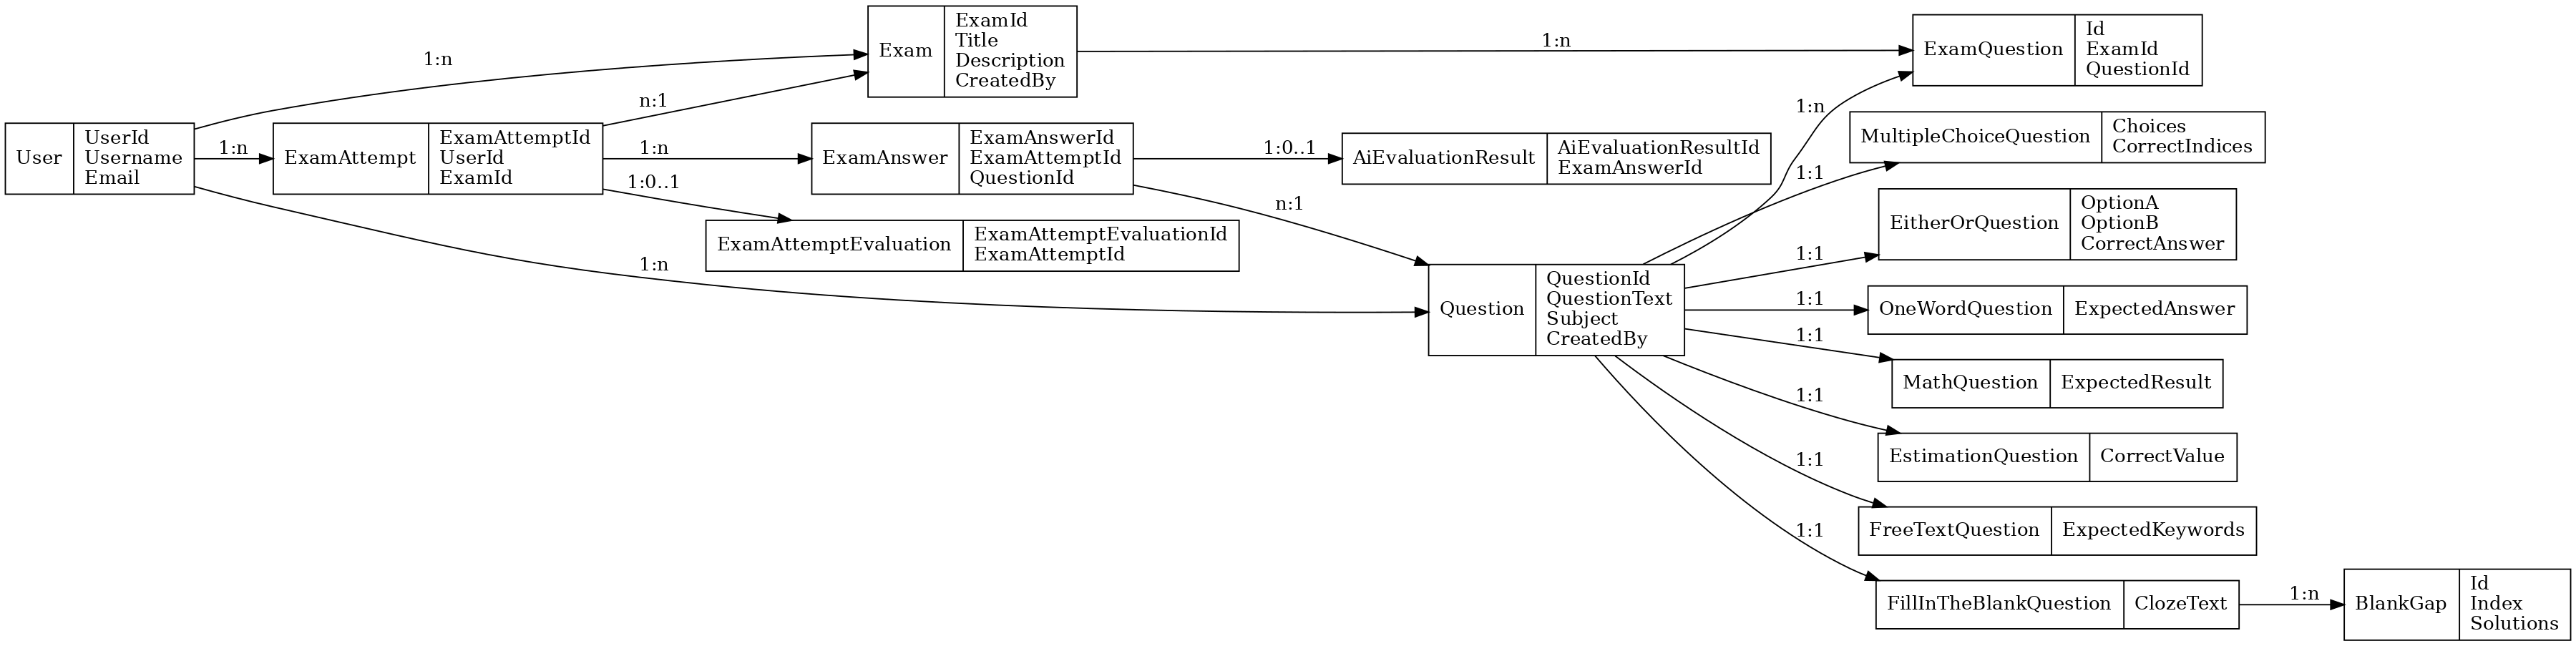
\includegraphics[width=1.1\textwidth]{Bilder/er_diagram_highres.png}
\caption{Entity-Relationship-Diagramm der GenAI-Bewertungsplattform}
\label{fig:erd}
\end{figure}
\vspace{1em}

Wie in Abbildung~\ref{fig:erd} dargestellt, bilden die Entitäten ein klar strukturiertes und normalisiertes Modell, das eine präzise Trennung zwischen Nutzerinteraktionen, Prüfungsstruktur, Antworten und Bewertungen ermöglicht. Diese Modularität ist entscheidend für die Wartbarkeit des Systems und unterstützt die kontinuierliche Weiterentwicklung. Die Struktur wurde im Verlauf des Projekts schrittweise erweitert, insbesondere im Hinblick auf die Differenzierung von Fragetypen und die Integration des generativen Bewertungssystems. Der aktuelle Stand bietet eine tragfähige Grundlage für zukünftige Erweiterungen wie Fortschrittsanalysen, adaptive Frageauswahl oder erweiterte Feedbackmechanismen.

\subsection{API-Kommunikation}
Die Kommunikation zwischen den verschiedenen Komponenten des Systems folgt dem Prinzip einer serviceorientierten Architektur (SOA) und basiert auf standardisierten RESTful Webservices. Diese Schnittstellen dienen nicht nur der Verbindung zwischen Frontend und Backend, sondern insbesondere auch der Integration externer KI-Dienste, im konkreten Fall der OpenAI-API zur automatisierten Bewertung von Freitext- und anderen offenen Antwortformaten.

\subsubsection{Interne Kommunikation (Frontend-Backend)}
Sobald ein Prüfungsversuch abgeschlossen wurde, werden die im Frontend eingegebenen Antworten als strukturierte Datenobjekte (SubmitExamAttemptDto) an das Backend gesendet. Diese enthalten neben den Antwortinhalten auch Metadaten wie Prüfungs- und Benutzer-IDs. Im Backend erfolgt zunächst die Speicherung der Antworten in der Datenbank. Anschließend werden sie zur Bewertung vorbereitet, indem die relevante Frage mitsamt ihrer Typ-spezifischen Konfiguration (z.B. Multiple-Choice-Optionen oder erwartete Ergebnisse) analysiert und mit den Benutzereinstellungen (Toleranz für Tippfehler, Groß-/Kleinschreibung, Schätztoleranz) angereichert wird.

\subsubsection{Externe Kommunikation (Backend-OpenAI API)}
Die anschließende Auswertung erfolgt durch die Integration der OpenAI-API. Für jede zu bewertende Antwort wird im Backend ein spezifisch strukturierter Prompt generiert, der aus der Frage, der Nutzereingabe, der erwarteten Lösung und den Bewertungseinstellungen besteht. Diese Informationen werden als Teil eines JSON-Objekts an die API gesendet. Der Aufruf erfolgt als HTTP-POST-Anfrage mit einem festgelegten Sprachmodell (z.B. gpt-4), wobei ein rollenbasierter Konversationsverlauf (system und user) verwendet wird, um dem Modell klare Bewertungsanweisungen zu geben.

Die API antwortet mit einer textbasierten Rückgabe, die ein JSON-Fragment enthält, bestehend aus einer numerischen Bewertung (score) im Bereich von 0 bis 1 sowie einem erklärenden Feedback. Das System extrahiert dieses JSON aus der Antwort mithilfe regulärer Ausdrücke und deserialisiert es anschließend in eine interne Bewertungsstruktur (AiEvaluationResult). Diese Ergebnisse werden der entsprechenden Nutzerantwort zugeordnet und persistent gespeichert.

\subsubsection{Sicherheitsaspekte und Architekturmerkmale}
Die API-Schlüssel für den Zugriff auf die OpenAI-API werden über die Konfigurationsdateien des Backends verwaltet und nicht im Quellcode hinterlegt. Die gesamte Kommunikation mit dem externen Dienst erfolgt verschlüsselt über HTTPS. Die REST-API ist durch rollenbasierte Zugriffskontrollen abgesichert, wobei alle prüfungsrelevanten Endpunkte Authentifizierung per JSON Web Token (JWT) voraussetzen.

\subsubsection{Zusammenfassung}
Die API-Kommunikation stellt die zentrale Brücke zwischen Nutzereingabe und KI-gestützter Bewertung dar. Sie erlaubt die dynamische Generierung von Bewertungen durch den OpenAI-Dienst und liefert eine flexible, semantisch fundierte Rückmeldung, die über klassische Antwort-Matching-Algorithmen weit hinausgeht. Die Entkopplung von Benutzeroberfläche, Bewertungskomponente und Speicherlogik ermöglicht eine klare Trennung von Zuständigkeiten, was sowohl die Wartbarkeit als auch die Erweiterbarkeit der Anwendung unterstützt.

\subsection{Teststrategie}

Die Qualitätssicherung des entwickelten Systems erfolgte durch eine systematische Kombination aus Unit-Tests, Integrationstests und explorativen manuellen Tests. Ziel dieser Strategie war es, die Funktionalität, Robustheit und Wartbarkeit sowohl der Backend- als auch der Frontend-Komponenten abzusichern.

\subsubsection{Backend-Tests mit xUnit}
Für das serverseitige System wurde ein umfassender Satz an Unit-Tests mit dem Framework \textit{xUnit} implementiert. Diese Tests prüfen die einzelnen Dienste, Controller und Validierungslogiken isoliert voneinander. Dabei werden Abhängigkeiten durch Mocking mithilfe der \textit{Moq}-Bibliothek ersetzt, um das Verhalten in kontrollierten Szenarien zu evaluieren. Der Fokus lag auf der Verifikation zentraler Funktionen wie der Benutzerregistrierung, Authentifizierung, Frage- und Prüfungsverwaltung sowie der korrekten Übergabe von Bewertungsanfragen an die generative KI-Schnittstelle. Durch gezielte Tests auf Fehlerszenarien, unautorisierte Zugriffe und ungültige Eingaben wurde eine hohe Fehlertoleranz sichergestellt. Ebenso wurden typische REST-Statuscodes wie 200 (OK), 400 (Bad Request) oder 401 (Unauthorized) validiert.

\subsubsection{Frontend-Komponententests mit Jasmine und Karma}
Im Frontend wurde für zentrale Komponenten (z.B. Prüfungsversuch, Frageeditor, Login) eine Testumgebung mit \textit{Jasmine} als Testframework und \textit{Karma} als Test-Runner eingerichtet. Ziel war es, das Verhalten von Angular-Komponenten in isolierten Testszenarien zu prüfen. Durch das Einbinden von Testmodulen wie dem \textit{HttpClientTestingModule} oder \textit{MatSnackBarModule} konnten auch komplexere Abhängigkeiten simuliert werden. Beispielsweise wurde überprüft, ob ein Timer korrekt initialisiert wird, wenn ein Zeitlimit gesetzt ist, oder ob Benutzerinteraktionen wie das Wechseln zwischen Fragen korrekt verarbeitet werden.

\subsubsection{Testabdeckung und Validierung}
Während die Backend-Tests eine nahezu vollständige Abdeckung der Geschäftslogik aufweisen, konzentrieren sich die Frontend-Tests gezielt auf kritische Benutzerinteraktionen. Besondere Beachtung fanden hier Logiken, die nicht unmittelbar über das UI testbar sind, wie die automatische Abgabe einer Prüfung bei Zeitüberschreitung. Derartige Funktionalitäten wurden gezielt durch asynchrone Testszenarien und Mock-Komponenten geprüft. Ergänzend zu den automatisierten Tests wurden manuelle Prüfungen durchgeführt, um visuelles Verhalten, Responsivität und korrekte Internationalisierung zu validieren.

\subsubsection{Bewertung}
Die gewählte Teststrategie stellt sicher, dass sowohl funktionale Anforderungen als auch Sicherheits- und Stabilitätsaspekte systematisch abgedeckt werden. Hervorzuheben ist die modulare Struktur des Codes, die das gezielte Testen einzelner Einheiten erleichtert. Die frühzeitige Einbindung von Tests im Entwicklungsprozess führte zu einer Reduktion typischer Integrationsfehler und erhöhter Wartbarkeit.

Insgesamt unterstützt die testgetriebene Entwicklung nicht nur die Sicherstellung der Softwarequalität, sondern trägt auch zu einer nachhaltig wartbaren Architektur bei.

\newpage

\section{Implementierung}
\subsection{Implementierung der Fragetypen}
Das System unterstützt eine Vielzahl didaktisch relevanter Fragetypen, die jeweils spezifische Anforderungen an Eingabelogik, Speicherung und Bewertung stellen. Die Umsetzung dieser Typen folgt dem Prinzip der Vererbung und Polymorphie. Eine abstrakte Basisklasse \texttt{Question} definiert gemeinsame Eigenschaften wie Fragetext, Thema, Ersteller und Zeitpunkt der Erstellung. Die konkreten Typen, \textit{MultipleChoice}, \textit{OneWord} oder \textit{FillInTheBlank}, leiten von dieser Klasse ab und erweitern sie um jeweils spezifische Attribute.

Die Datenspeicherung erfolgt über eine relationale Datenbankstruktur, wobei Entity Framework Core (EF Core) als Object-Relational-Mapper verwendet wird. Jeder Fragetyp wird als eigene Entität mit Table-per-Hierarchy-Strategie abgebildet. Dies ermöglicht eine typensichere und performante Abfrage sowie eine saubere Trennung der Geschäftslogik im Backend.

Die zentrale API zur Verwaltung der Fragen ist im \texttt{QuestionsController} implementiert und stellt Endpunkte für das Erstellen, Bearbeiten, Abrufen und Löschen von Fragen bereit. Diese API verarbeitet eingehende Daten über dedizierte DTO-Klassen (Data Transfer Objects) und konvertiert sie mittels eines zentralen \texttt{QuestionMapper} in die jeweilige Entität. Diese Trennung ermöglicht eine flexible Erweiterbarkeit und schützt die interne Logik vor unbeabsichtigter Manipulation durch externe Clients.

Die konkrete Benutzerinteraktion erfolgt im Angular-Frontend. Die Eingabemaske zur Erstellung neuer Fragen reagiert dynamisch auf die Auswahl des Fragetypen wie in Abbildung \ref{fig:Fragenübersicht} zu sehen ist. Je nach gewählter Option werden passende Eingabefelder angezeigt, z.B. Checkboxen für Multiple-Choice-Fragen, ein strukturierter Lückentexteditor für Fill-in-the-Blank oder ein Freitextfeld mit erwarteten Schlüsselwörtern. Die Formularlogik basiert auf \texttt{Reactive Forms} und ermöglicht so eine strukturierte Validierung der Eingaben vor dem Absenden. Unvollständige oder inkonsistente Eingaben führen zu kontextbezogenen Fehlermeldungen, was die Datenqualität erhöht.

\begin{figure}[H]
    \centering
    \includegraphics[width=0.7\textwidth]{Bilder/Fragenübersicht.png}
    \caption{Fragenübersicht}
    \label{fig:Fragenübersicht}
\end{figure}

Der Fragetyp „FillInTheBlank“ stellt dabei eine besondere Herausforderung dar: Hier wird ein Platzhaltertext eingegeben, in dem Lücken durch \{\{0\}\}, \{\{1\}\} usw. markiert sind. Diese Lücken werden im Backend mit einer Liste gültiger Lösungen (\texttt{BlankGap}) verknüpft, die über eine Eins-zu-Viele-Relation zur zugehörigen Frage verwaltet werden. Die Datenstruktur ermöglicht beliebig viele Lücken und Lösungsmöglichkeiten pro Frage. Die Validierung stellt sicher, dass zu jeder Lücke mindestens eine gültige Lösung angegeben ist.

Die Abbildung der Fragetypen auf Benutzeroberfläche, Datenmodell und Persistenzschicht folgt einem durchgängigen Architekturkonzept, das eine Erweiterung um weitere Typen jederzeit ermöglicht. Die Implementierung erlaubt es, Fragen als polymorphe Objekte zu behandeln, wodurch Funktionen wie API-Endpunkte, Serialisierung und KI-basierte Bewertung typübergreifend konsistent bleiben.

\subsection{Integration der generativen KI-Bewertung}
Die zentrale Innovation des Projekts besteht in der automatisierten Auswertung von Prüfungsantworten mittels generativer KI. Zu diesem Zweck wurde die OpenAI-API in das Bewertungssystem integriert, um die Analyse und Bewertung von Nutzerantworten, insbesondere bei offenen Fragetypen, semantisch zu fundieren und didaktisch zu unterstützen. Ziel war es, die Limitierungen klassischer Regelverfahren zu überwinden, die lediglich auf formale Übereinstimmung prüfen, und stattdessen ein Bewertungssystem zu schaffen, das kontextuelle Bedeutung, Ausdrucksvielfalt und sprachliche Varianz adäquat erfassen kann.

Technisch erfolgt die Anbindung der generativen KI im Rahmen des Backends durch den Dienst \texttt{OpenAiService}, der sämtliche Kommunikation mit der OpenAI-API kapselt. Für jede Antwort wird dynamisch ein strukturierter Prompt generiert, der neben der ursprünglichen Frage auch die Nutzerantwort, die korrekte Lösung sowie individuelle Bewertungseinstellungen enthält (vgl. Abb. \ref{fig:Prompt}). Diese umfassen unter anderem Parameter zur Toleranz gegenüber Tippfehlern, zur Groß- und Kleinschreibung sowie zur Schätzgenauigkeit (vgl. Abb. \ref{fig:Prompt2}). Der Prompt wird über ein rollenbasiertes Dialogmodell an das KI-System übermittelt, welches eine Bewertung im JSON-Format zurückliefert. Diese Bewertung besteht aus einem numerischen Score zwischen 0 und 1 sowie einem erklärenden Feedbacktext, der den Nutzern Rückmeldung über ihre Antwortqualität gibt.

\begin{figure}[H]
    \centering
    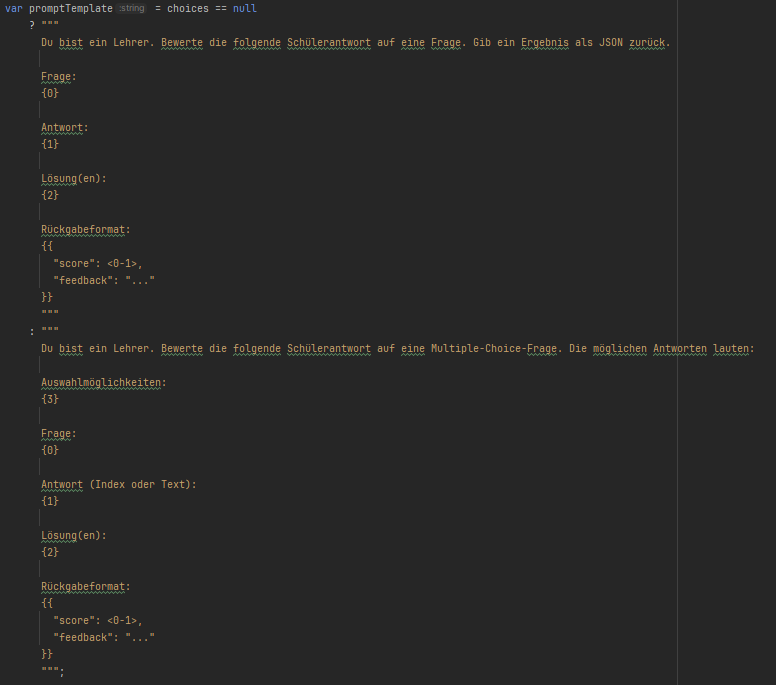
\includegraphics[width=1\textwidth]{Bilder/Prompt.png}
    \caption{Prompt}
    \label{fig:Prompt}
\end{figure}

\begin{figure}[H]
    \centering
    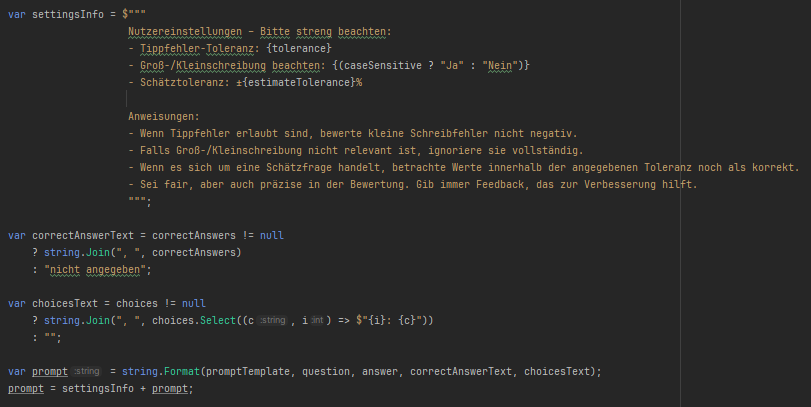
\includegraphics[width=1\textwidth]{Bilder/Prompt2.png}
    \caption{Nutzereinstellungen Prompt}
    \label{fig:Prompt2}
\end{figure}

Die Antworten werden durch den \texttt{ExamAttemptRepository} zunächst persistiert und anschließend in einem mehrstufigen Bewertungsprozess analysiert. Der \texttt{ExamScoringService} übernimmt dabei die inhaltliche Aufbereitung der Daten und passt die Bewertungslogik an den jeweiligen Fragetyp an. So werden bei Multiple-Choice-Fragen die ausgewählten Indizes in textuelle Optionen umgewandelt, bei Lückentexten die Struktur der Gaps berücksichtigt und bei Freitextantworten explizite Schlüsselwörter extrahiert. Alle diese Informationen fließen in die Bewertung durch die generative KI ein. Das Ergebnis wird in der Entität \texttt{AiEvaluationResult} gespeichert und durch eine zusammenfassende Evaluation auf Versuchsebene (\texttt{ExamAttemptEvaluation}) ergänzt.

Der Bewertungsprozess ist vollständig asynchron umgesetzt und wird unmittelbar nach Abgabe eines Prüfungsversuchs ausgelöst. Innerhalb weniger Sekunden steht den Teilnehmenden eine detaillierte Rückmeldung zur Verfügung. Diese umfasst sowohl Einzelbewertungen pro Frage als auch eine aggregierte Abschlussbewertung samt Bestehensinformation. Die Rückgabe erfolgt im \texttt{ExamAttemptResultDto}, welches im Frontend visualisiert wird. Ergänzt wird das System durch ein Fortschritts-Dashboard, das die bisherigen Ergebnisse übersichtlich zusammenfasst.

Die Nutzung generativer KI für Bewertungszwecke stellt nicht nur einen technologischen Fortschritt dar, sondern erfordert zugleich ein reflektiertes Verständnis ihrer Einsatzgrenzen. Wie in Kapitel \ref{sec:hintergrund} dargestellt, sind Modelle wie GPT-4 nicht deterministisch, d.h. identische Anfragen können zu unterschiedlichen Bewertungen führen. Um dieser Herausforderung zu begegnen, wurden strukturierte Prompts, konsistente Bewertungsanweisungen und standardisierte Antwortformate eingeführt, um die Reproduzierbarkeit und Nachvollziehbarkeit der Ergebnisse zu erhöhen. Darüber hinaus muss jederzeit eine manuelle Nachprüfung durch Lehrpersonen möglich sein, um sicherzustellen, dass die pädagogische Verantwortung nicht vollständig an die KI abgegeben wird, insbesondere bei ihrem Einsatz in realen Lernsituationen.

Zusammenfassend lässt sich festhalten, dass die Integration der generativen KI eine bedeutende Erweiterung der Bewertungslogik darstellt. Sie ermöglicht erstmals eine automatisierte Auswertung auch bei Freitexten, komplexen Argumentationen und schätzbaren Werten, ein Bereich, der bislang weitgehend manueller Prüfung vorbehalten war. Durch den modularen Aufbau der Bewertungsarchitektur lässt sich das System künftig auf weitere KI-Modelle oder differenzierte Bewertungslogiken ausweiten.

\subsection{Datenbankstruktur und Datenmodelle}
Die Implementierung der Datenbankstruktur stellt ein zentrales Fundament für die gesamte Anwendungsarchitektur dar. Grundlage bildet eine relationale PostgreSQL-Datenbank, welche über das ORM-Framework Entity Framework Core (\acs{EF}) in das .NET-Backend integriert wurde. Die Persistenzschicht basiert auf einem Typenmodell, das stark an die inhaltliche Struktur der Anwendung angelehnt ist: Fragen, Prüfungen, Benutzer, Versuche und KI-basierte Bewertungen sind als jeweils eigene Entitäten modelliert und bilden eine logisch nachvollziehbare Trennung der fachlichen Verantwortung.

Ein zentrales Element stellt die polymorphe Modellierung der Fragetypen dar. Die abstrakte Basisklasse \texttt{Question} definiert gemeinsame Attribute wie \texttt{QuestionText}, \texttt{Subject}, \texttt{CreatedBy} sowie Metadaten zur Erstellung. Darauf aufbauend implementiert das System eine Table-per-Type (TPT) Vererbungsstrategie, bei der spezialisierte Fragetypen (z.B. \texttt{MultipleChoiceQuestion}, \texttt{FreeTextQuestion}, \texttt{MathQuestion}, \texttt{FillInTheBlankQuestion}) jeweils eigene Tabellen erhalten, die mit der Haupttabelle \texttt{Questions} verknüpft sind. Dies ermöglicht eine saubere Trennung, typensichere Validierung und eine gezielte Abfrage der jeweiligen Fragetypen.

Besondere Beachtung findet die Modellierung komplexer Fragetypen wie der Lückentextfragen. Diese bestehen aus einem Text mit Platzhaltern (\texttt{ClozeText}), der durch die Entität \texttt{FillInTheBlankQuestion} repräsentiert wird. Die dazugehörigen Lücken (\texttt{BlankGaps}) sind über eine 1:n-Relation verbunden und enthalten jeweils eine Liste möglicher Lösungen im JSON-Format. Diese flexible Modellierung erlaubt die Definition beliebig vieler Lücken und lässt sich in der KI-Bewertung differenziert auswerten.

Die Entität \texttt{Exam} bildet Prüfungseinheiten ab, die wiederum über eine Zwischentabelle \texttt{ExamQuestion} mit den Fragen verknüpft sind. Die Zuordnung erfolgt inklusive Positionsinformation (\texttt{Order}), sodass eine feste Reihenfolge der Fragen gewahrt bleibt. Die 1:n-Verbindung zu \texttt{ExamAttempt} dokumentiert alle von Nutzern gestarteten Versuche. Jeder Versuch speichert neben Metadaten (Startzeit, Abgabezeitpunkt, Userreferenz) auch die gegebenen Antworten in Form der Entität \texttt{ExamAnswer}.

Jede Antwort enthält entweder eine freie Texteingabe (\texttt{TextAnswer}) oder eine Auswahl (\texttt{SelectedIndices}) und referenziert sowohl Frage als auch Versuch. Die Bewertung erfolgt durch eine 1:1-Relation zur Entität \texttt{AiEvaluationResult}, welche durch das KI-System generiert und in der Datenbank abgelegt wird. Enthalten sind dabei sowohl die Punktzahl (Score), ein boolesches Richtig/Falsch-Flag als auch ein qualifiziertes Feedback zur Antwort.

Auf Ebene des gesamten Versuchs werden aggregierte Bewertungen in der Entität \\ \texttt{ExamAttemptEvaluation} zusammengefasst. Sie enthält die durchschnittliche Punktzahl, das Bestehenskriterium sowie ein summarisches Feedback. Diese Struktur ermöglicht sowohl eine individuelle Auswertung pro Frage als auch eine übergeordnete Lernstandsdiagnose.

Neben der Modellierung wurde auch besonderer Wert auf Performance und Skalierbarkeit gelegt. So sind kritische Felder wie \texttt{UserId} und \texttt{Subject} mit Datenbankindizes versehen, um effiziente Abfragen für statistische Auswertungen zu ermöglichen. JSON-Felder für Mehrfachantworten und Lückenlösungen ermöglichen eine flexible, aber strukturierte Speicherung komplexer Daten.

Zusammenfassend lässt sich festhalten, dass die Datenbankstruktur nicht nur als Speicher für Prüfungsdaten dient, sondern als logisches Abbild der Bewertungslogik verstanden werden kann. Ihre polymorphe und relationale Struktur unterstützt sowohl die Validität der Bewertungen als auch die Nachvollziehbarkeit einzelner Schritte in der Prüfungsanalyse. Die Trennung zwischen Datenhaltung, Bewertung und Nutzerinteraktion schafft dabei eine solide Grundlage für Erweiterungen wie Lernverlaufsanalysen oder adaptive Feedbacksysteme.

\subsection{Entwicklung der Benutzeroberfläche}
Die Entwicklung der Benutzeroberfläche erfolgte mit dem Ziel, eine intuitive, reaktionsschnelle und barrierearme Anwendung zu schaffen, die sowohl Funktionalität als auch Nutzerfreundlichkeit vereint. Technologisch basiert das Frontend auf dem Framework Angular in Kombination mit TypeScript, SCSS und der Bibliothek \texttt{ngx-translate} zur Internationalisierung. Neben den klassischen Anforderungen an ein responsives Webdesign stand insbesondere die Interaktion mit komplexen Formularen, dynamischen Fragetypen sowie der KI-gestützten Bewertung im Fokus der Oberflächengestaltung.

Die Benutzeroberfläche ist komponentenbasiert strukturiert, wobei jede Teilfunktionalität in einer eigenen Angular-Komponente gekapselt ist. Zentrale Bestandteile sind u.a. das 	\texttt{ProfileComponent} zur Verwaltung von Benutzereinstellungen, Fortschrittsanzeige und erstellten Inhalten, das \texttt{QuestionsComponent} zur Frageerstellung sowie das \\	\texttt{ExamAttemptComponent} für die Durchführung von Prüfungen. Diese Struktur erleichtert nicht nur die Wiederverwendbarkeit von Komponenten, sondern auch deren gezieltes Testen und Wartung.

Die Benutzerinteraktion erfolgt vorwiegend über Reactive Forms, wodurch eine reaktive Validierung und formularspezifische Logik implementiert werden konnte. Dynamische UI-Elemente, wie z.B. Fragetyp-spezifische Eingabemasken, werden dabei kontextabhängig eingeblendet. So werden bei der Erstellung einer 	\texttt{MultipleChoice}-Frage Eingabefelder für Antwortmöglichkeiten und Checkboxen zur Markierung korrekter Antworten angezeigt, während bei 	\texttt{FillInTheBlank}-Fragen ein Lückentext-Editor mit individuell konfigurierbaren Antwortfeldern zum Einsatz kommt. Der Aufbau komplexer Fragetypen wird somit für Nutzer nachvollziehbar und visuell unterstützt (vgl. Abb. \ref{fig:Fragenübersicht}).

Ein weiteres Kernelement ist die Prüfungsdurchführung im 	\texttt{ExamAttemptComponent}, welche die gestellten Fragen in einem seitenintegrierten Navigationslayout darstellt (vgl. Abb \ref{fig:exam}). Der Fortschritt der Nutzer wird visuell in einer Sidebar angezeigt. Ein integrierter Timer überwacht verbleibende Bearbeitungszeit. Die Antworten werden formularbasiert erfasst und dynamisch an die jeweilige Fragetypik angepasst: So sind bei 	\texttt{Math}- und 	\texttt{Estimation}-Fragen numerische Eingaben vorgesehen, während 	\texttt{FreeText}-Fragen ein mehrzeiliges Textfeld bieten. Lückentextfragen erlauben die Eingabe von Einzelbegriffen in sequenziell angeordneten Feldern, deren Anzahl automatisch aus dem Platzhaltertext abgeleitet wird.

\begin{figure}[H]
    \centering
    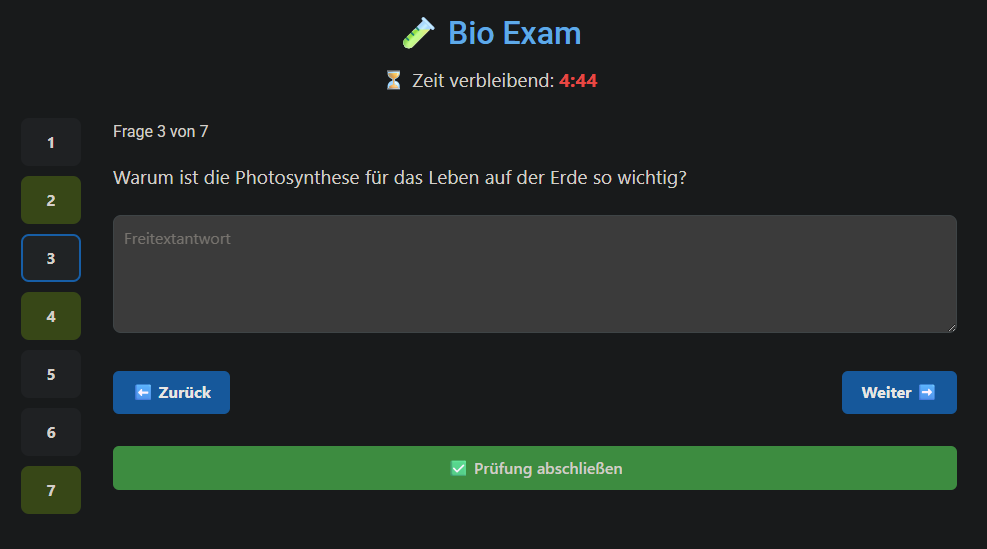
\includegraphics[width=1\textwidth]{Bilder/Exam.png}
    \caption{Exam UI}
    \label{fig:exam}
\end{figure}

Die Benutzeroberfläche unterstützt darüber hinaus die Visualisierung der Ergebnisse nach Abschluss einer Prüfung. Im 	\texttt{ExamResultComponent} werden die Einzelergebnisse jeder Frage inklusive der von der KI erzeugten Bewertung, Beurteilung und Feedback ausgegeben (vgl. Abb. \ref{fig:ergebnis}). Durch visuelle Hervorhebung korrekter und inkorrekter Antworten sowie einer übersichtlichen Darstellung der Gesamtleistung wird der Lerneffekt der Nutzer gezielt gefördert.

\begin{figure}[H]
    \centering
    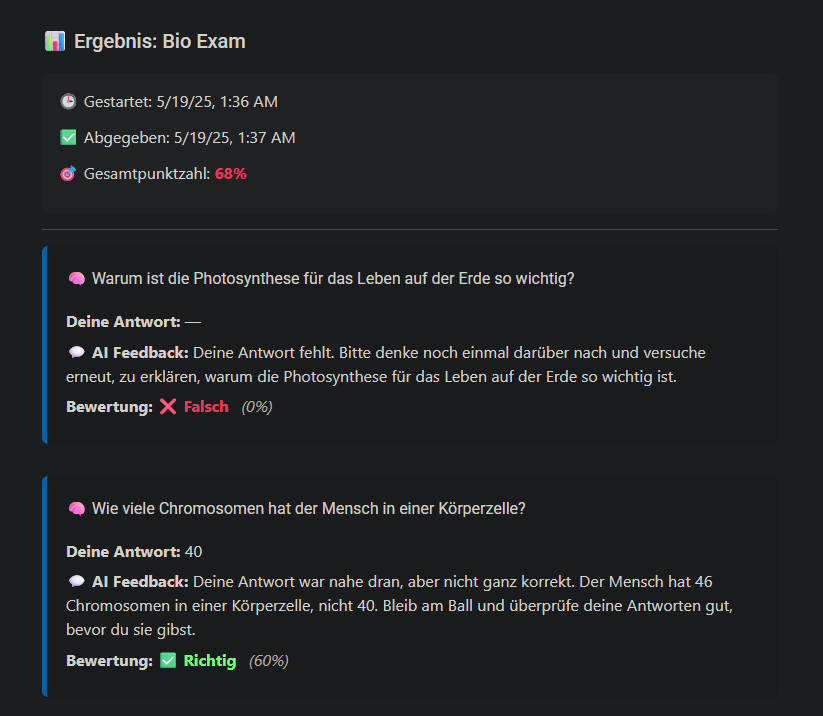
\includegraphics[width=1\textwidth]{Bilder/Ergebnis.png}
    \caption{Ergebnis einer Prüfung}
    \label{fig:ergebnis}
\end{figure}

Das Profilmodul (	\texttt{ProfileComponent}) erlaubt zusätzlich die Verwaltung individueller Benutzereinstellungen. Hier können unter anderem Bewertungstoleranzen, Groß-/Kleinschreibung sowie Spracheinstellungen konfiguriert und dauerhaft gespeichert werden (vgl. Abb. \ref{fig:settings}). Die Implementierung eines 	\texttt{HttpInterceptor} gewährleistet dabei die sichere Übertragung von Authentifizierungsdaten und Token-basierten Zugriffsschutz für geschützte Ressourcen.

Insgesamt zeichnet sich die Benutzeroberfläche durch eine hohe funktionale Tiefe, eine modulare Architektur und eine klare Trennung von Präsentations- und Logikschicht aus. Durch die Kombination von Angular, responsivem Design, asynchroner Kommunikation mit dem Backend sowie gezielten UX-Elementen wie Progress-Indikatoren, Filterfunktionen und Bestätigungsdialogen wurde eine praxisnahe und didaktisch wirksame Lernoberfläche realisiert.

\begin{figure}[H]
    \centering
    \includegraphics[width=1\textwidth]{Bilder/settings.png}
    \caption{Benutzereinstellungen}
    \label{fig:settings}
\end{figure}
\newpage

\section{Ergebnisse und Diskussion}

Im Rahmen dieses Projekts wird ein webbasiertes System zur automatisierten Bewertung offener und geschlossener Antworten in digitalen Lernumgebungen konzipiert, implementiert und umfassend evaluiert. Die zentralen Ergebnisse zeigen, dass durch den gezielten Einsatz generativer KI-Technologien eine signifikante Steigerung der Bewertungsqualität im Vergleich zu klassischen Algorithmen erreicht werden kann, insbesondere bei Fragetypen, die sprachliche Varianz, Kontextsensitivität oder flexible Toleranzbereiche erfordern.

Ein zentrales Ziel besteht darin, die technische Machbarkeit und funktionale Tragfähigkeit eines MVP zu demonstrieren, das sich durch modulare Erweiterbarkeit, Benutzerfreundlichkeit und eine serviceorientierte Architektur auszeichnet. Diese Zielsetzung wird durch die Entwicklung eines voll funktionsfähigen Systems erfüllt, das Antworten über verschiedene Fragetypen hinweg analysieren, bewerten und mit individuellem Feedback versehen kann. Die Integration der OpenAI-API in die Backend-Logik ermöglicht eine flexible Bewertungsstrategie, die sowohl formale als auch semantische Aspekte berücksichtigt.

Die Vergleichsstudie zwischen verschiedenen generativen Modellen offenbart Unterschiede hinsichtlich Genauigkeit, Feedbackqualität und Bewertungsstabilität. Modelle wie GPT-4o Mini überzeugen durch hohe Konsistenz, ausgeprägtes Kontextverständnis und didaktisch verwertbares Feedback, während leichtere Modelle mit Vorteilen bei Kosten und Geschwindigkeit punkten, jedoch bei komplexeren Aufgaben an qualitative Grenzen stoßen. Diese Ergebnisse unterstreichen, dass die Wahl des Modells entscheidend von der intendierten Anwendungssituation abhängen muss, eine Erkenntnis, die insbesondere für künftige produktive Implementierungen von hoher Relevanz ist.

Neben der technischen Implementierung stehen auch didaktische und ethische Fragestellungen im Mittelpunkt der Untersuchung. Die nicht-deterministische Natur generativer Modelle, die Möglichkeit von Halluzinationen sowie begrenzte Nachvollziehbarkeit der Bewertungsergebnisse machen deutlich, dass ein KI-gestütztes Bewertungssystem keine vollständig autonome Prüfungsinstanz darstellen kann. Die Ergebnisse zeigen jedoch, dass durch strukturierte Prompts, kontrollierte Bewertungskriterien und transparente Rückmeldestrukturen ein hoher Grad an Zuverlässigkeit erzielt werden kann, sofern eine menschliche Überprüfung in kritischen Fällen weiterhin gewährleistet ist.

Auf Grundlage dieser Resultate lässt sich feststellen, dass der entwickelte Prototyp eine belastbare Grundlage für zukünftige Anwendungen bietet. Die Architektur erlaubt eine Erweiterung um zusätzliche Fragetypen, verbesserte Analysemechanismen und adaptive Feedbackprozesse. Gleichzeitig verdeutlichen die Ergebnisse, dass bei allen technologischen Fortschritten die pädagogische Einbettung, die Kontrolle durch Lehrpersonen und die Sensibilisierung für mögliche systemische Verzerrungen unerlässlich bleiben. Die Diskussion dieser Aspekte liefert wesentliche Impulse für die Weiterentwicklung des Systems und die Integration generativer KI in reale Bildungsprozesse. (vgl. \cite{luckin})

\subsection{Zusammenfassung der Implementierungsergebnisse}
Die im Rahmen dieses Projekts umgesetzte Systemarchitektur erfüllt in vollem Umfang die Zielsetzung eines funktionalen MVP zur automatisierten Antwortbewertung unter Einsatz generativer KI-Technologien. Die Implementierung zeigt, dass durch eine klar strukturierte Fullstack-Architektur auf Basis von Angular (Frontend) und ASP.NET Core (Backend) eine leistungsfähige, modular erweiterbare Plattform realisierbar ist, die sowohl funktionale als auch nicht-funktionale Anforderungen erfüllt.

Auf funktionaler Ebene konnten alle zentralen Fragetypen erfolgreich abgebildet und technisch umgesetzt werden: Multiple-Choice-, Ein-Wort-, Rechen-, Entweder/Oder-, Schätz-, Lückentext- sowie Freitextfragen. Die Implementierung beruht auf einer polymorphen Datenmodellierung, welche die Typenvielfalt konsistent handhabbar macht und eine differenzierte Bewertung ermöglicht. Über die REST-basierte API-Schnittstelle erfolgt die nahtlose Kommunikation zwischen Frontend, Backend und externem KI-Dienst. Die dynamische Prompt-Generierung, angereichert durch Nutzereinstellungen wie Toleranzlevel oder Groß-/Kleinschreibungsoptionen, ermöglicht eine kontextsensitive und semantisch fundierte Bewertung durch das angebundene Sprachmodell (OpenAI GPT).

Die Integration der generativen KI in die Bewertungskette erwies sich als zentraler Innovationsschritt. Sie erlaubt nicht nur eine Bewertung jenseits statischer Regelwerke, sondern generiert zugleich differenziertes, sprachlich angepasstes Feedback für die Nutzer. Dies trägt wesentlich zur didaktischen Qualität und zur Akzeptanz des Systems bei. Die Bewertungslogik ist asynchron implementiert und vollständig entkoppelt vom Frontend, was eine gute Skalierbarkeit und Erweiterbarkeit garantiert.

Die Benutzeroberfläche wurde responsiv und benutzerzentriert gestaltet. Sie unterstützt sowohl die Erstellung, Bearbeitung und Verwaltung von Prüfungen als auch die Durchführung durch Lernende. Fortschrittsanzeigen, Timerfunktionen, ein konfigurierbares Bewertungsprofil und eine Ergebnisübersicht mit Feedbackvisualisierung sind vollständig integriert. Technologisch wurde auf eine komponentenbasierte Umsetzung geachtet, wodurch eine hohe Wiederverwendbarkeit und Testbarkeit einzelner UI-Elemente sichergestellt ist.

Auf Persistenzebene stellt die relationale Datenbankstruktur mit klar definierten Entitäten für Nutzer, Prüfungen, Antworten und Bewertungen eine solide Grundlage für Datenintegrität und Nachvollziehbarkeit dar. Durch gezielte Normalisierung, Indexierung und den Einsatz von JSON-Feldern bei komplexeren Datenstrukturen wie Lückenlösungen konnte eine gute Balance zwischen Performance und Flexibilität erreicht werden.

Ergänzt wird die technische Realisierung durch eine durchdachte Teststrategie. Die Kombination aus Unit- und Integrationstests im Backend (xUnit, Moq) sowie Komponententests im Frontend (Jasmine, Karma) gewährleistet eine hohe Systemstabilität und Fehlertoleranz. Explorative Tests validierten zudem die Benutzerfreundlichkeit und Responsivität.

Insgesamt belegt die Implementierung, dass ein KI-gestütztes Bewertungssystem unter Berücksichtigung technischer, didaktischer und ethischer Anforderungen realisierbar ist. Der vorliegende Prototyp bietet ein belastbares Fundament für produktive Anwendungsszenarien und lässt sich durch seinen modularen Aufbau gezielt um weiterführende Funktionen, wie adaptive Lernpfade, multimodale Eingabeformate oder erweiterte Feedbackstrategien, ergänzen.

\subsection{Herausforderungen bei der Entwicklung}

Die Entwicklung des KI-gestützten Bewertungssystems stellte eine Reihe spezifischer Herausforderungen dar, die sowohl technischer als auch organisatorischer Natur waren. Diese ergaben sich aus der Komplexität der eingesetzten Technologien, den Eigenschaften generativer Sprachmodelle sowie den Rahmenbedingungen des Projekts, das als Ein-Personen-Entwicklung unter begrenzten Ressourcen realisiert wurde.

\subsubsection{Nichtdeterminismus und Inkonsistenz generativer KI-Ausgaben}
Eine der zentralen technischen Herausforderungen bestand in der nichtdeterministischen Natur der generativen Sprachmodelle. Selbst bei identischen Eingaben und streng strukturierten Prompts lieferten die Modelle teils abweichende Punktzahlen und Begründungen. Diese Inkonsistenzen erschwerten nicht nur die Vergleichbarkeit zwischen verschiedenen Modellen, sondern auch die systematische Evaluierung einzelner Bewertungen. In einigen Fällen traten sogenannte Halluzinationen auf, also sachlich falsche oder unplausible Rückmeldungen, obwohl die Antwort formal korrekt oder zumindest nachvollziehbar war. Um diesem Problem zu begegnen, wurden strukturierte Bewertungsformate und standardisierte Prompts im Backend eingeführt. Dennoch bleibt der stochastische Charakter generativer Modelle ein fundamentaler Unsicherheitsfaktor, der in der praktischen Anwendung berücksichtigt werden muss.

Die nicht deterministische Ergebnisstruktur der KI-Modelle erschwerte auch den fairen Vergleich zwischen verschiedenen Anbietern. Während sich Unterschiede in Bezug auf Preisstruktur und API-Zugänglichkeit relativ objektiv erheben ließen, war die Bewertung von Konsistenz und Qualität der Ausgaben durch zufallsbedingte Schwankungen beeinflusst. Um dennoch belastbare Aussagen zu treffen, wurde jedes Modell mehrfach mit identischen Prompts getestet. Modelle mit hoher Variabilität und häufigen Halluzinationen konnten so identifiziert werden, was zu einer Fokussierung auf solche mit möglichst stabiler Antwortqualität führte.

\subsubsection{Begrenzte Ressourcen und ihr Einfluss auf die Modellbewertung}

Die Nutzung generativer KI-Systeme über APIs verursacht insbesondere bei der Testdatengenerierung, Promptoptimierung und Modellauswahl einen erheblichen Tokenverbrauch und damit verbundene Kosten. Da im Rahmen dieser Studienarbeit nur ein begrenztes Budget zur Verfügung stand, erfolgten die Tests zunächst direkt über die jeweiligen Chat-Oberflächen der KI-Modelle und nicht über eine API-Anbindung. Aus diesem Grund wurden vorrangig kostenfreie oder kostengünstige Modelle eingesetzt, was jedoch mit funktionalen Einschränkungen verbunden war. Erst nach einer vergleichenden Analyse hinsichtlich Effizienz und Genauigkeit wurde ein geeignetes Modell ausgewählt, für das anschließend ein kostenpflichtiger API-Zugang lizenziert wurde. Potenzielle Ungenauigkeiten zwischen den Ergebnissen der Chat-Oberflächen und dem späteren API-Zugriff werden wissentlich in Kauf genommen.

\subsubsection{Entwicklung unter begrenzten Ressourcen}

Trotz einer umfassenden initialen Planung und Dokumentation war die Entwicklung durch zahlreiche iterative Anpassungen geprägt. Als Einzelentwickler war es notwendig, alle Rollen, vom Architekturdesign über das Frontend, Backend, Datenbankmodellierung bis hin zur Integration und Testdurchführung, selbst zu übernehmen. Dies führte zu einem hohen Koordinationsaufwand und erforderte ein hohes Maß an Flexibilität, insbesondere bei der Reaktion auf unvorhergesehene technische Probleme oder konzeptionelle Anpassungen.

Zur strukturierten Planung und Nachverfolgung des Projektfortschritts wurde GitHub nicht nur zur Versionsverwaltung, sondern auch zur Dokumentation und Projektorganisation genutzt. Unter anderem kamen ein Software Requirements Specification (SRS) sowie ein Kanban-Board zum Einsatz, um Anforderungen in Form von Tickets zu erfassen, Aufgaben zu priorisieren und die iterative Entwicklung systematisch zu steuern.

Zudem mussten verschiedene Technologien und Frameworks parallel erlernt und angewendet werden, was den Entwicklungsprozess verlangsamte, aber zugleich zu einem tiefgreifenden Verständnis der gesamten Systemarchitektur beitrug.

Obwohl zu Beginn des Projekts ein umfangreiches Architektur- und Anforderungsmodell ausgearbeitet wurde, erwies sich der Bedarf an nachträglichen Anpassungen als unvermeidbar. Beispielsweise mussten einige Fragetypen um zusätzliche Parameter erweitert werden, um die Bewertungslogik flexibler zu gestalten. Ebenso mussten Datenbankstrukturen angepasst und neu migriert werden, sobald sich im Testbetrieb neue funktionale Anforderungen ergaben. Diese Änderungen erforderten eine saubere Trennung von Komponenten, eine konsequente Nutzung von Interfaces und eine hohe Testabdeckung, um Regressionen zu vermeiden.

\subsubsection{Technologische Komplexität durch Schnittstellenintegration}

Die Anbindung externer Dienste, insbesondere der OpenAI-API, stellte eine weitere Herausforderung dar. Die Kommunikation erforderte nicht nur eine sorgfältige Konstruktion von Prompts, sondern auch eine robuste Fehlerbehandlung, Logging und Sicherheitsmaßnahmen zur API-Schlüsselverwaltung. Die Extraktion und Interpretation der Antwortdaten im JSON-Format erwies sich als fehleranfällig, da nicht alle Rückgaben dem erwarteten Schema entsprachen. Hier war der Einsatz regulärer Ausdrücke und zusätzlicher Validierungslogik notwendig, um fehlerhafte oder unvollständige Rückgaben korrekt zu verarbeiten.

\newpage

\section{Zukünftige Arbeiten und Erweiterungsmöglichkeiten}
Die Grundlagen, die durch das Entwickeln eines KI-gestützten Bewertungssystems gesetzt wurden, stellen ein belastbares Fundament für weiterführende Forschung und Entwicklungsarbeiten im Kontext digitaler Lernumgebungen dar. Das entwickelte MVP demonstriert eindrücklich das Potenzial generativer KI zur flexiblen und kontextsensitiven Analyse von Antworten. Dennoch verbleiben zahlreiche Erweiterungsmöglichkeiten, die sowohl funktionale als auch didaktische und technologische Dimensionen adressieren. Im Folgenden werden zentrale Entwicklungsperspektiven systematisch ausgeführt.

\subsection{Adaptive Lernpfade}
Ein zentrales Ziel künftiger Weiterentwicklungen besteht in der Implementierung adaptiver Lernpfade. Diese verfolgen das Konzept, Lerninhalte individuell an den Kompetenzstand und Lernfortschritt der jeweiligen Nutzer anzupassen. Die bereits implementierte Sammlung nutzerspezifischer Bewertungsdaten bildet eine geeignete Ausgangsbasis für ein solches System. Aufbauend auf aggregierten Auswertungen ließe sich ein regelbasiertes oder KI-gestütztes Empfehlungssystem entwickeln, das gezielte Übungsvorschläge generiert, Wissenslücken identifiziert und Folgeaufgaben dynamisch auswählt. Perspektivisch denkbar ist auch die Integration diagnostischer Algorithmen, die Lernenden nach bestimmten Fehlertypen oder kognitiven Mustern differenzierte Fördermaterialien zuweisen.

Didaktisch erfordert ein solches System die Modellierung von Lernzielen und Kompetenzstufen. Die Kombination aus generativer KI zur Bewertung und klassischer Kompetenzmodellierung zur Steuerung eröffnet hier ein hybrides System, das sowohl inhaltlich flexibel als auch curricular fundiert agieren kann. Technisch bedarf es dazu zusätzlicher Datenbankstrukturen, Nutzungsanalysen und Entscheidungslogik, die auf bestehenden Bewertungsergebnissen aufbauen und diese in semantisch kohärente Lernpfade überführen.

\subsection{Integration von Sprach- und Bilderkennung}
Eine mögliche Erweiterung des Bewertungssystems liegt in der Integration zusätzlicher Eingabeformate wie Sprache und Bilder. Aktuell basiert das System ausschließlich auf Textantworten, was jedoch bestimmte Nutzergruppen oder Aufgabentypen einschränken kann. Durch die Einbindung von Spracherkennung könnten Lernende ihre Antworten auch mündlich geben. Die gesprochenen Inhalte würden automatisch in Text umgewandelt und anschließend wie bisher durch die KI bewertet. Dies wäre hilfreich für junge Nutzer, Personen mit Schreibschwierigkeiten oder in sprachbasierten Lernfächern wie Fremdsprachen.

Ebenso denkbar ist die Erweiterung um Bilderkennung, zur Bewertung von handschriftlichen Rechenwegen oder Skizzen. Ein solches System könnte eingescannte oder fotografierte Antworten analysieren und daraus relevante Informationen extrahieren. Dies eröffnet neue Möglichkeiten in Fächern wie Mathematik, Physik oder Kunst, in denen visuelle Elemente eine zentrale Rolle spielen. Die Umsetzung erfordert zwar zusätzliche technische Komponenten, würde jedoch den Anwendungsbereich und die Barrierefreiheit des Systems erweitern.

\subsection{Mehrsprachigkeit}
Ein weiterer zentraler Baustein zukünftiger Entwicklungen ist die Umsetzung umfassender Mehrsprachigkeit. Zwar wurde das System bereits mit Unterstützung für Sprachpakete im Frontend konzipiert, jedoch beschränkt sich die KI-gestützte Bewertung aktuell auf deutschsprachige Inhalte. Perspektivisch sollte das System um eine sprachübergreifende Verarbeitung erweitert werden, sodass sowohl Eingaben als auch Prompts in verschiedenen Sprachen verarbeitet werden können. Dies betrifft nicht nur die Benutzeroberfläche, sondern insbesondere die Bewertungslogik und das Feedback der KI.

Technologisch ist dies mit GPT-basierten Modellen prinzipiell umsetzbar, bedarf jedoch gezielter Promptgestaltung, Sprachspezifikation und ggf. einer Validierung sprachspezifischer Bewertungslogiken. Ergänzend sollten auch kulturelle Unterschiede in Ausdrucksweisen, Argumentationsstrukturen und sprachlicher Variation berücksichtigt werden, um eine faire und kontextsensible Bewertung über Sprachgrenzen hinweg sicherzustellen.

\subsection{Erweiterung des Rollen- und Rechtemanagements}

Im derzeitigen MVP wurde bewusst auf ein differenziertes Rollenmodell verzichtet. Für produktive Einsatzszenarien ist jedoch die Einführung spezifischer Rollen, Administrator, Lehrkräfte und Lernende, unabdingbar. Künftige Arbeiten sollten daher ein Rollen- und Rechtemanagement vorsehen, das differenzierte Zugriffsrechte, Prüfungsberechtigungen und Feedbackoptionen ermöglicht. Auch die Anbindung an bestehende Lernmanagementsysteme könnte in diesem Zusammenhang verfolgt werden, um das System nahtlos in bestehende Bildungsinfrastrukturen zu integrieren.

\newpage

\section{Fazit}
Die vorliegende Arbeit befasst sich mit der Entwicklung und Evaluation eines webbasierten Systems zur KI-gestützten Bewertung von Antworten in digitalen Lernumgebungen. Aufbauend auf einer fundierten Analyse technischer, didaktischer und architektonischer Anforderungen wurde ein Prototyp realisiert, der die Möglichkeiten generativer KI nutzbar macht, um flexible, kontextbezogene und nachvollziehbare Bewertungen zu erzeugen. Im abschließenden Kapitel werden die erreichten Ziele zusammengefasst, die Bedeutung der Ergebnisse im bildungstechnologischen Kontext eingeordnet und Perspektiven für weiterführende Entwicklungen aufgezeigt. Dabei steht nicht nur die technische Machbarkeit, sondern auch die pädagogische Tragfähigkeit im Zentrum der Betrachtung.

\subsection{Erfüllung der Projektziele}
Die im Projekt verfolgten Zielsetzungen werden umfassend erreicht. Das entwickelte System bildet ein MVP, das generative KI erfolgreich zur automatisierten Bewertung unterschiedlicher Fragetypen einsetzt. Durch die Integration einer leistungsfähigen Sprachmodell-API gelingt es, eine Bewertung umzusetzen, die formale Abweichungen, semantische Nuancen und kontextuelle Bedeutung berücksichtigt. Die Architektur des Systems ist modular, wartbar und für zukünftige Erweiterungen vorbereitet. Sowohl die funktionale Breite als auch die technische Tiefe der Implementierung erfüllen die definierten Anforderungen in vollem Umfang.

Neben der technischen Realisierbarkeit bestätigt das Projekt auch die Praxistauglichkeit der Lösung. Prüfungen lassen sich zuverlässig erstellen, durchführen und automatisch bewerten. Die Nutzer erhalten unmittelbar differenziertes Feedback, das auf individuelle Antwortmuster eingeht. Die Kombination aus Backend-Logik, datenbankgestützter Persistenz und responsivem Frontend führt zu einem kohärenten System, das nicht nur in Testumgebungen, sondern auch im realen Einsatzkontext bestehen kann.

\subsection{Bedeutung der Ergebnisse}
Die Ergebnisse des Projekts besitzen sowohl technische als auch bildungspraktische Relevanz. Aus technologischer Perspektive zeigt die Untersuchung, dass generative KI-Modelle in der Lage sind, eine semantisch fundierte und nachvollziehbare Bewertung zu liefern; ein erheblicher Fortschritt gegenüber klassischen Algorithmen. Die Evaluation verschiedener Modelle verdeutlicht, dass nicht nur Genauigkeit, sondern auch Feedbackqualität, Konsistenz und ökonomische Faktoren bei der Auswahl der Technologie zu berücksichtigen sind.

Didaktisch eröffnet die automatisierte, inhaltlich differenzierte Bewertung neue Möglichkeiten in digitalen Lernumgebungen. Lernende profitieren von personalisierten Rückmeldungen, die nicht auf starren Regeln, sondern auf inhaltlicher Analyse basieren. Gleichzeitig behalten Lehrende die Möglichkeit zur Nachkontrolle und Qualitätssicherung. Das System fördert so nicht nur die Effizienz, sondern auch die Fairness und Transparenz des Bewertungsprozesses.

Darüber hinaus liefern die Ergebnisse einen fundierten Ausgangspunkt für weitere Forschung. Die Kombination klassischer Bewertungslogik mit generativen Verfahren bietet ein hybrides Modell, das in unterschiedlichen pädagogischen Kontexten adaptierbar ist. Insbesondere die Flexibilität der Bewertungseinstellungen legt den Grundstein für eine individualisierte Lernpfadsteuerung.

\subsection{Ausblick}
Die im Projekt erarbeitete Lösung stellt eine belastbare Grundlage für zukünftige Entwicklungen dar. Perspektivisch lässt sich das System um adaptive Lernpfade erweitern, die Nutzerleistungen systematisch analysieren und darauf basierende Inhalte vorschlagen. Die bestehende Datenstruktur ermöglicht eine solche Erweiterung ohne grundlegende Umstrukturierung.

Auch die Integration multimodaler Eingabeformate stellt eine naheliegende Weiterentwicklung dar. Die Verarbeitung gesprochener Antworten oder bildlicher Inhalte eröffnet neue Anwendungsfelder, etwa in der Grundbildung oder in fachspezifischen Disziplinen. Ebenso ist die umfassende Umsetzung von Mehrsprachigkeit ein wichtiger Schritt zur internationalen Skalierbarkeit der Plattform.

Langfristig bietet das System das Potenzial, über klassische Prüfungsanwendungen hinaus als lernunterstützendes Werkzeug zu fungieren. Durch gezielte Rückmeldungen, Fortschrittsanalysen und individualisierte Aufgabenstellungen kann ein digitales Lernökosystem entstehen, das die Potenziale generativer KI konsequent in den Dienst des Lernens stellt. Die Ergebnisse des Projekts zeigen, dass die technische, didaktische und ethische Integration solcher Systeme machbar und gestaltungsfähig ist, vorausgesetzt, sie erfolgt reflektiert und verantwortungsbewusst.

\newpage

\section{Anhang}
\label{anhang}
\appendix


\section{Prompts}

\subsection{Multiple-Choice Prompts}

\textbf{Frage:} [In welchem Teil der Pflanzenzelle findet die Photosynthese statt?] \\
\textbf{Antwort:} [Zellkern] \\
\textbf{Antwort Typ:} [Multiple-Choice] \\
\textbf{Parameter von Typen:} [\\
Antwortmöglichkeiten:[Zellkern, Mitochondrien, Chloroplasten, Ribosomen] \\
] \\
\textbf{Erwartete richtige Antwort:} [Chloroplasten] \\
\textbf{Bewertungskriterien:} \\
Entspricht die Antwort der Lösung? \\
Antwort bitte in diesem Format: \\
\{ \\
"Punktzahl": X, \\
"Begründung": "..." \\
\}

\vspace{1em}

\textbf{Frage:} [Wie lautet die Hauptstadt von Frankreich?] \\
\textbf{Antwort:} [Paris] \\
\textbf{Antwort Typ:} [Multiple-Choice] \\
\textbf{Parameter von Typen:} [\\
Antwortmöglichkeiten:[Berlin, Paris, Madrid, Prag] \\
] \\
\textbf{Erwartete richtige Antwort:} [Paris] \\
\textbf{Bewertungskriterien:} \\
Entspricht die Antwort der Lösung? \\
Antwort bitte in diesem Format: \\
\{ \\
"Punktzahl": X, \\
"Begründung": "..." \\
\}

\subsection{Ein-Wort-Antworten Prompts}

\textbf{Frage:} [Wie heißt die chemische Formel für Wasser?] \\
\textbf{Antwort:} [H2O] \\
\textbf{Antwort Typ:} [Ein-Wort-Antwort] \\
\textbf{Parameter von Typen:} [] \\
\textbf{Erwartete richtige Antwort:} [H$_2$O] \\
\textbf{Bewertungskriterien:} \\
Ist die Antwort korrekt? \\
Erlaube Rechtschreibfehler, so lange sie die Antwort nicht zu stark ändern \\
Synonyme, die im Kontext korrekt sind, sollen auch akzeptiert werden \\
Antwort bitte in diesem Format: \\
\{ \\
"Punktzahl": X, \\
"Begründung": "..." \\
\}

\vspace{1em}

\textbf{Frage:} [Wer schrieb das Buch „Faust“?] \\
\textbf{Antwort:} [Göthe] \\
\textbf{Antwort Typ:} [Ein-Wort-Antwort] \\
\textbf{Parameter von Typen:} [] \\
\textbf{Erwartete richtige Antwort:} [Goethe] \\
\textbf{Bewertungskriterien:} \\
Ist die Antwort korrekt? \\
Erlaube Rechtschreibfehler, so lange sie die Antwort nicht zu stark ändern \\
Synonyme, die im Kontext korrekt sind, sollen auch akzeptiert werden \\
Antwort bitte in diesem Format: \\
\{ \\
"Punktzahl": X, \\
"Begründung": "..." \\
\}

\vspace{1em}

\textbf{Frage:} [Wie nennt man das größte Organ des menschlichen Körpers?] \\
\textbf{Antwort:} [Leber] \\
\textbf{Antwort Typ:} [Ein-Wort-Antwort] \\
\textbf{Parameter von Typen:} [] \\
\textbf{Erwartete richtige Antwort:} [Haut] \\
\textbf{Bewertungskriterien:} \\
Ist die Antwort korrekt? \\
Erlaube Rechtschreibfehler, so lange sie die Antwort nicht zu stark ändern \\
Synonyme, die im Kontext korrekt sind, sollen auch akzeptiert werden \\
Antwort bitte in diesem Format: \\
\{ \\
"Punktzahl": X, \\
"Begründung": "..." \\
\}

\subsection{Rechenaufgaben Prompts}

\textbf{Frage:} [Ein Schüler hat 12 Äpfel. Er möchte sie gleichmäßig auf 4 Schüsseln verteilen. Wie viele Äpfel kommen in jede Schüssel?] \\
\textbf{Antwort:} [3,5] \\
\textbf{Antwort Typ:} [Rechenaufgabe] \\
\textbf{Parameter von Typen:} [] \\
\textbf{Erwartete richtige Antwort:} [3] \\
\textbf{Bewertungskriterien:} \\
Erkennt die KI korrekte und falsche Antworten? \\
Kann die KI mathematische Aufgaben (Division) lösen oder bewerten? \\
Wird auf richtige Einheiten, Zahlenformat und Vollständigkeit geachtet? \\
Antwort bitte in diesem Format: \\
\{ \\
"Punktzahl": X, \\
"Begründung": "..." \\
\}

\vspace{1em}

\textbf{Frage:} [Ein Rechteck hat eine Länge von 12cm und eine Breite von 7cm. Wie groß ist der Flächeninhalt?] \\
\textbf{Antwort:} [96cm] \\
\textbf{Antwort Typ:} [Rechenaufgabe] \\
\textbf{Parameter von Typen:} [] \\
\textbf{Erwartete richtige Antwort:} [84cm²] \\
\textbf{Bewertungskriterien:} \\
Wurde die Rechnung korrekt durchgeführt? \\
Ist die Antwort korrekt, auch wenn keine Einheit angegeben wurde? \\
Werden alternative Formate akzeptiert? (z.B. „84cm“ vs. „84“) \\
Antwort bitte in diesem Format: \\
\{ \\
"Punktzahl": X, \\
"Begründung": "..." \\
\}

\subsection{Entweder-Oder-Fragen Prompts}

\textbf{Frage:} [Ist der Eiffelturm höher als der Kölner Dom?] \\
\textbf{Antwort:} [Nein] \\
\textbf{Antwort Typ:} [Entweder/Oder] \\
\textbf{Parameter von Typen:} [] \\
\textbf{Erwartete richtige Antwort:} [Ja] \\
\textbf{Bewertungskriterien:} \\
Ist die Antwort inhaltlich korrekt? \\
Werden alternative Schreibweisen berücksichtigt (z.B. „ja“, „Ja, natürlich“, „nein“)? \\
Sind kleinere sprachliche Abweichungen akzeptabel? \\
Antwort bitte in diesem Format: \\
\{ \\
"Punktzahl": X, \\
"Begründung": "..." \\
\}

\subsection{Schätzfragen Prompts}

\textbf{Frage:} [Wie hoch ist der Eiffelturm?] \\
\textbf{Antwort:} [350m] \\
\textbf{Antwort Typ:} [Schätzfrage] \\
\textbf{Parameter von Typen:} [ \\
Akzeptabler Bereich: [±10\%] \\
] \\
\textbf{Erwartete richtige Antwort:} [330m] \\
\textbf{Bewertungskriterien:} \\
Wird eine Toleranz bei der Bewertung berücksichtigt? \\
Gibt die KI eine Begründung für die Bewertung? \\
Kann die KI die Abweichung berechnen oder muss der Bereich vorgegeben werden? \\
Antwort bitte in diesem Format: \\
\{ \\
"Punktzahl": X, \\
"Begründung": "..." \\
\}

\subsection{Lückentextfragen Prompts}

\textbf{Frage:} [Die Photosynthese findet in den \_\_\_ der Pflanzenzelle statt. Dabei wird mit Hilfe von \_\_\_ und Lichtenergie \_\_\_ in Glukose umgewandelt.] \\
\textbf{Antwort:} [Chloroplasten, Wasser, Kohlendioxid] \\
\textbf{Antwort Typ:} [Lückentextfrage] \\
\textbf{Parameter von Typen:} [ \\
Antwortmöglichkeiten:[Wasser, Sonne, Chloroplasten, Zellkern, Kohlendioxid, Sauerstoff] \\
] \\
\textbf{Erwartete richtige Antwort:} [Chloroplasten, Wasser, Kohlendioxid] \\
\textbf{Bewertungskriterien:} \\
Sind alle Lücken korrekt und fachlich richtig ausgefüllt? \\
Werden alternative Begriffe akzeptiert (z.B. „CO$_2$“ statt „Kohlendioxid“)? \\
Werden kleinere Schreibfehler toleriert? \\
Kann die KI teilweise korrekte Antworten differenziert bewerten? \\
Antwort bitte in diesem Format: \\
\{ \\
"Punktzahl": X, \\
"Begründung": "..." \\
\}

\vspace{1em}

\textbf{Frage:} [Im Jahr \_\_\_ begann der Zweite Weltkrieg mit dem Überfall Deutschlands auf \_\_\_. Der Krieg endete im Jahr \_\_\_ mit der Kapitulation \_\_\_.] \\
\textbf{Antwort:} [1936, Polen, 1945, Russlands] \\
\textbf{Antwort Typ:} [Lückentextfrage] \\
\textbf{Parameter von Typen:} [ \\
Antwortmöglichkeiten:[1936, 1939, 1945, Polen, Russlands, Deutschlands, Tschechien] \\
] \\
\textbf{Erwartete richtige Antwort:} [1939, Polen, 1945, Deutschlands] \\
\textbf{Bewertungskriterien:} \\
Sind alle Lücken historisch korrekt ausgefüllt? \\
Werden alternative Schreibweisen akzeptiert (z.B. „BRD“ oder „NS-Deutschland“ für „Deutschland“)? \\
Können kleine Tippfehler oder Datumsformate (z.B. „'39“) toleriert werden? \\
Gibt es eine Teilbewertung bei teilweise richtigen Angaben? \\
Antwort bitte in diesem Format: \\
\{ \\
"Punktzahl": X, \\
"Begründung": "..." \\
\}

\subsection{Freitextantworten Prompts}

\textbf{Frage:} [Erkläre, warum der Treibhauseffekt sowohl für das Leben auf der Erde notwendig als auch in seiner verstärkten Form problematisch ist.] \\
\textbf{Antwort:} [Der Treibhauseffekt sorgt dafür, dass die Erde warm genug bleibt, damit Leben existieren kann. Wenn er aber zu stark wird, weil zu viele Gase wie CO$_2$ ausgestoßen werden, wird es zu heiß, was zum Klimawandel führt.] \\
\textbf{Antwort Typ:} [Freitextantwort] \\
\textbf{Parameter von Typen:} [] \\
\textbf{Erwartete richtige Antwort:} [Der natürliche Treibhauseffekt ist entscheidend für das Leben auf der Erde, da er die durchschnittliche Temperatur auf einem Niveau hält, das flüssiges Wasser und damit Leben ermöglicht. In seiner verstärkten Form – verursacht durch den Anstieg menschengemachter Treibhausgase wie CO$_2$ und Methan – führt er jedoch zur globalen Erwärmung. Diese bringt schwerwiegende Folgen mit sich, etwa häufigere Extremwetterereignisse, das Abschmelzen von Gletschern und den Anstieg des Meeresspiegels.] \\
\textbf{Bewertungskriterien:} \\
Wird der Unterschied zwischen natürlichem und verstärktem Treibhauseffekt korrekt dargestellt? \\
Werden die positiven und negativen Aspekte nachvollziehbar erklärt? \\
Sind wissenschaftlich relevante Begriffe korrekt verwendet (z.B. „Treibhausgase“, „globale Erwärmung“)? \\
Ist die Antwort logisch aufgebaut und sprachlich klar formuliert? \\
Gibt es sachliche Fehler, Auslassungen oder vereinfachende Verkürzungen? \\
Wird bei teilrichtigen Antworten differenziert bewertet? \\
Antwort bitte in diesem Format: \\
\{ \\
"Punktzahl": X, \\
"Begründung": "..." \\
\}

\section{KI Antworten}

\subsection{ChatGPT}

\subsubsection{Multiple-Choice}

\textbf{Photosynthese}
\begin{quote}
\{"Punktzahl": 0,\\
"Begründung": "Die gegebene Antwort 'Zellkern' ist falsch, da die Photosynthese in den Chloroplasten stattfindet. Die richtige Antwort wäre 'Chloroplasten' gewesen."\}
\end{quote}

\textbf{Hauptstadt Frankreich}
\begin{quote}
\{"Punktzahl": 100,\\
"Begründung": "Die gegebene Antwort 'Paris' entspricht genau der erwarteten richtigen Antwort. Daher wird die volle Punktzahl vergeben."\}
\end{quote}

\subsubsection{Ein-Wort-Antworten}

\textbf{Wasser}
\begin{quote}
\{"Punktzahl": 100,\\
"Begründung": "Die Antwort 'H2O' ist korrekt und entspricht der chemischen Formel für Wasser. Der Unterschied zur erwarteten Antwort 'H₂O' liegt nur in der Schreibweise der tiefgestellten Zahl, was keinen inhaltlichen Unterschied macht."\}
\end{quote}

\textbf{Goethe}
\begin{quote}
\{"Punktzahl": 90,\\
"Begründung": "Die Antwort ist fast korrekt, jedoch enthält sie einen kleinen Rechtschreibfehler ('Göthe' statt 'Goethe'). Da die Bedeutung der Antwort nicht verändert wird und klar erkennbar ist, was gemeint war, gibt es nur einen kleinen Abzug."\}
\end{quote}

\textbf{Haut}
\begin{quote}
\{"Punktzahl": 0,\\
"Begründung": "Die gegebene Antwort 'Leber' ist leider falsch. Das größte Organ des menschlichen Körpers ist die 'Haut'. Bitte überprüfe die Antwort noch einmal."\}
\end{quote}

\subsubsection{Rechenfragen}

\textbf{Äpfel}
\begin{quote}
\{"Punktzahl": 10,\\
"Begründung": "Die Antwort '3,5' ist leider falsch, da 12 Äpfel gleichmäßig auf 4 Schüsseln verteilt genau 3 Äpfel pro Schüssel ergibt. Die Division 12 ÷ 4 = 3 ist eine einfache Rechenaufgabe, bei der die Antwort eine ganze Zahl sein muss, weil man keine halben Äpfel verteilt, wenn nichts dergleichen erwähnt ist. Gut wäre es, die Grundrechenarten sicher zu beherrschen."\}
\end{quote}

\textbf{Fläche}
\begin{quote}
\{"Punktzahl": 10,\\
"Begründung": "Die Antwort ist leider falsch. Der Flächeninhalt eines Rechtecks berechnet sich aus Länge mal Breite, also 12cm × 7cm = 84cm². Die Antwort 96cm ist daher ein Rechenfehler. Außerdem fehlt die korrekte Einheit (cm²). Achte beim nächsten Mal darauf, die richtige Formel zu verwenden und das Ergebnis zu überprüfen."\}
\end{quote}

\subsubsection{Entweder-oder-Fragen}

\textbf{Eiffelturm}
\begin{quote}
\{"Punktzahl": 0,\\
"Begründung": "Die Antwort ist inhaltlich falsch – der Eiffelturm ist mit etwa 330 Metern deutlich höher als der Kölner Dom mit rund 157 Metern. Da es sich um eine Entweder/Oder-Frage handelt, kommt es allein auf die inhaltliche Richtigkeit an, alternative Formulierungen sind hier nicht relevant. Achte beim nächsten Mal einfach darauf, kurz zu prüfen, welche Struktur wirklich höher ist – das hilft schon enorm!"\}
\end{quote}

\subsubsection{Schätzfrage}

\textbf{Höhe}
\begin{quote}
\{"Punktzahl": 80,\\
"Begründung": "Deine Antwort liegt mit 350m nur knapp außerhalb des akzeptablen Bereichs von ±10\% (297m bis 363m). Allerdings wäre der richtige Wert für den Eiffelturm etwa 330m, was deine Schätzung ziemlich nah dran macht. Gute Arbeit – kleine Abweichung, aber insgesamt eine solide Schätzung!"\}
\end{quote}

\begin{quote}
\{"Punktzahl": 91,\\
"Begründung": "Deine Schätzung von 350m liegt nur 6,1\% über der erwarteten Höhe von 330m und damit im akzeptablen Bereich von ±10\%. Die Antwort ist also sehr nah dran – gut geschätzt! Für eine perfekte Punktzahl hätte eine noch genauere Angabe (z.B. 330m oder 331m) gesorgt."\}
\end{quote}

\subsubsection{Lückentextfragen}

\textbf{Zelle}
\begin{quote}
\{"Punktzahl": 100,\\
"Begründung": "Super gemacht! Alle Lücken wurden korrekt und fachlich richtig ausgefüllt: Die Photosynthese findet in den Chloroplasten statt, dabei wird Wasser zusammen mit Kohlendioxid und Lichtenergie in Glukose umgewandelt. Es gibt nichts zu beanstanden!"\}
\end{quote}

\textbf{WWII}
\begin{quote}
\{"Punktzahl": 50,\\
"Begründung": "Du hast zwei von vier Lücken korrekt ausgefüllt – 'Polen' und '1945' sind richtig. Der Beginn des Zweiten Weltkriegs war jedoch 1939, nicht 1936. Auch endete der Krieg mit der Kapitulation Deutschlands, nicht Russlands. Es ist gut, dass du Polen und das Endjahr korrekt erkannt hast, aber achte bitte auf die historischen Details, besonders bei solch zentralen Ereignissen."\}
\end{quote}

\subsubsection{Freitextfragen}

\textbf{Treibhauseffekt}
\begin{quote}
\{"Punktzahl": 80,\\
"Begründung": "Die Antwort ist klar formuliert und trifft die grundlegende Aussage: Der Treibhauseffekt ist wichtig für das Leben, kann aber in seiner verstärkten Form problematisch sein. Der Unterschied zwischen natürlichem und verstärktem Treibhauseffekt wird angedeutet, aber nicht explizit benannt. Begriffe wie 'CO₂' und 'Klimawandel' sind korrekt verwendet, jedoch fehlt die Verwendung zentraler wissenschaftlicher Begriffe wie 'globale Erwärmung' oder die Nennung weiterer Treibhausgase (z.B. Methan). Auch konkrete Folgen wie Extremwetterereignisse oder Meeresspiegelanstieg bleiben unerwähnt. Insgesamt eine gute, aber etwas vereinfachte Antwort."\}
\end{quote}

\subsection{DeepSeek}

\subsubsection{Multiple-Choice}

\textbf{Photosynthese}
\begin{quote}
\{"Punktzahl": 0,\\
"Begründung": "Die gegebene Antwort 'Zellkern' entspricht nicht der erwarteten richtigen Antwort 'Chloroplasten'. Die Photosynthese findet in den Chloroplasten der Pflanzenzelle statt, nicht im Zellkern."\}
\end{quote}

\textbf{Hauptstadt Frankreich}
\begin{quote}
\{"Punktzahl": 100,\\
"Begründung": "Die gegebene Antwort 'Paris' entspricht der erwarteten richtigen Antwort 'Paris'. Die Antwort ist korrekt und vollständig."\}
\end{quote}

\subsubsection{Ein-Wort-Antworten}

\textbf{Wasser}
\begin{quote}
\{"Punktzahl": 100,\\
"Begründung": "Die gegebene Antwort 'H2O' ist korrekt und entspricht der erwarteten richtigen Antwort 'H₂O'. Die Verwendung von '2' anstelle des tiefgestellten '₂' ist in diesem Kontext akzeptabel, da es die chemische Formel nicht verändert und die Lesbarkeit nicht beeinträchtigt. Die Antwort ist somit vollständig richtig."\}
\end{quote}

\textbf{Goethe}
\begin{quote}
Mehrfaches testen führte zu stark abweichenden Ergebnissen!!! \\
Mal 80 Punkte, mal 50 Punkte

\{"Punktzahl": 80,\\
"Begründung": "Die Antwort 'Göthe' ist fast korrekt, enthält jedoch einen kleinen Rechtschreibfehler. Der korrekte Name des Autors ist 'Goethe'. Der Fehler ändert die Bedeutung der Antwort nicht wesentlich, da die Aussprache und der Kontext klar erkennbar sind. Dennoch ist die Schreibweise nicht vollständig korrekt, daher gibt es einen kleinen Punktabzug."\}
\end{quote}

\textbf{Haut}
\begin{quote}
\{"Punktzahl": 0,\\
"Begründung": "Die Antwort 'Leber' ist leider nicht korrekt. Das größte Organ des menschlichen Körpers ist die Haut. Die Leber ist zwar ein wichtiges Organ, aber nicht das größte. Achte darauf, bei solchen Fragen die genaue Bezeichnung des gesuchten Organs zu verwenden."\}
\end{quote}

\subsubsection{Rechenfragen}

\textbf{Äpfel}
\begin{quote}
\{"Punktzahl": 0,\\
"Begründung": "Die gegebene Antwort '3,5' ist falsch, da 12 Äpfel gleichmäßig auf 4 Schüsseln verteilt genau 3 Äpfel pro Schüssel ergeben. Es gibt keine halben Äpfel in dieser Aufgabe. Achte darauf, dass du bei solchen Aufgaben immer prüfst, ob das Ergebnis sinnvoll und ganzzahlig ist."\}
\end{quote}

\textbf{Fläche}
\begin{quote}
\{"Punktzahl": 33,\\
"Begründung": "Die Rechnung wurde nicht korrekt durchgeführt, da der Flächeninhalt eines Rechtecks mit Länge 12 cm und Breite 7 cm 84 cm² beträgt, nicht 96 cm. Die Einheit wurde zwar angegeben, aber in der falschen Form (cm statt cm²). Achte darauf, die Formel für den Flächeninhalt (Länge × Breite) richtig anzuwenden und die korrekte Einheit zu verwenden."\}
\end{quote}

\subsubsection{Entweder-oder-Fragen}

\textbf{Eiffelturm}
\begin{quote}
\{"Punktzahl": 0,\\
"Begründung": "Die Antwort ist inhaltlich nicht korrekt. Der Eiffelturm (ca. 330 m) ist tatsächlich höher als der Kölner Dom (ca. 157 m). Achte bei Entweder/Oder-Fragen darauf, die Fakten richtig zu überprüfen, bevor du antwortest."\}
\end{quote}

\subsubsection{Schätzfrage}

\textbf{Höhe - Antwort 1}
\begin{quote}
\{"Punktzahl": 75,\\
"Begründung": "Deine Schätzung von 350 m liegt knapp außerhalb des akzeptablen Bereichs (±10\% der tatsächlichen Höhe von 330 m, also 297 m bis 363 m). Die Abweichung beträgt etwa 6\% über dem oberen Limit. Für eine bessere Bewertung solltest du dich möglichst nah am erwarteten Wert orientieren. Trotzdem war die Schätzung schon recht nah dran!"\}
\end{quote}

\textbf{Höhe - Antwort 2}
\begin{quote}
\{"Punktzahl": 100,\\
"Begründung": "Die Antwort liegt innerhalb des akzeptablen Bereichs von ±10\%. Die tatsächliche Höhe des Eiffelturms beträgt 330 Meter. Eine Abweichung von 20 Metern liegt innerhalb der Toleranz."\}
\end{quote}

Zwei komplett unterschiedliche Ausgaben bei gleicher Eingabe!

\subsubsection{Lückentextfrage}

\textbf{Zelle}
\begin{quote}
\{"Punktzahl": 100,\\
"Begründung": "Perfekt! Alle Lücken wurden korrekt und fachlich genau ausgefüllt. Du hast die richtigen Begriffe 'Chloroplasten', 'Wasser' und 'Kohlendioxid' gewählt, die genau den biologischen Prozess der Photosynthese beschreiben. Weiter so!"\}
\end{quote}

\textbf{WWII}
\begin{quote}
\{"Punktzahl": 50,\\
"Begründung": "Die Antwort enthält zwei richtige und zwei falsche Angaben. Richtig sind: Polen als angegriffenes Land und 1945 als Kriegsende. Die Fehler: Der Krieg begann 1939 (nicht 1936) und endete mit der Kapitulation Deutschlands (nicht Russlands). Historisch wichtige Daten solltest du noch genauer lernen. Die Hälfte der Antworten war aber korrekt!"\}
\end{quote}

\subsubsection{Freitextfragen}

\textbf{Treibhauseffekt}
\begin{quote}
\{"Punktzahl": 80,\\
"Begründung": "Deine Antwort erklärt die Grundlagen des Treibhauseffekts gut und nennt die wichtigsten Punkte: die lebenswichtige Funktion des natürlichen Effekts und die Probleme durch den verstärkten Effekt. Du hast die zentrale Rolle von CO₂ und den Klimawandel korrekt erwähnt. Zur Verbesserung könntest du noch etwas präziser werden (z.B. konkrete Folgen wie Extremwetter nennen) und wissenschaftliche Begriffe wie 'globale Erwärmung' konsequenter verwenden. Insgesamt aber eine klare und weitgehend vollständige Erklärung!"\}
\end{quote}

\subsection{Gemini}

\subsubsection{Multiple-Choice}

\textbf{Photosynthese}
\begin{quote}
\{"Punktzahl": 0,\\
"Begründung": "Die Photosynthese findet in den Chloroplasten statt, nicht im Zellkern. Der Zellkern ist für die Speicherung und Verarbeitung der genetischen Information zuständig."\}
\end{quote}

\textbf{Hauptstadt Frankreich}
\begin{quote}
\{"Punktzahl": 100,\\
"Begründung": "Die Antwort 'Paris' ist die korrekte Hauptstadt von Frankreich und entspricht somit der erwarteten richtigen Antwort."\}
\end{quote}

\subsubsection{Ein-Wort-Antworten}

\textbf{Wasser}
\begin{quote}
\{"Punktzahl": 100,\\
"Begründung": "Die Antwort ist perfekt! Die chemische Formel für Wasser ist H₂O (mit tiefgestellter 2). Deine Antwort H2O ist zwar nicht ganz korrekt formatiert, aber da es sich um eine Ein-Wort-Antwort handelt und die Bedeutung klar ist, gebe ich dir trotzdem die volle Punktzahl. Super gemacht!"\}
\end{quote}

\textbf{Goethe}
\begin{quote}
\{"Punktzahl": 90,\\
"Begründung": "Fast perfekt! Die Antwort ist inhaltlich richtig, aber der Nachname wird im Deutschen üblicherweise 'Goethe' geschrieben, nicht 'Göthe'. Da es sich aber nur um einen kleinen Rechtschreibfehler handelt, der die Bedeutung nicht verfälscht, gibt es fast die volle Punktzahl. Sehr gut!"\}
\end{quote}

\textbf{Haut}
\begin{quote}
\{"Punktzahl": 0,\\
"Begründung": "Die Antwort ist leider falsch. Das größte Organ des menschlichen Körpers ist die Haut und nicht die Leber. Die Leber ist zwar ein sehr wichtiges Organ und auch das größte innere Organ, aber die Haut übertrifft sie in ihrer Fläche um ein Vielfaches. Daher ist die Antwort 'Leber' nicht korrekt."\}
\end{quote}

\subsubsection{Rechenfragen}

\textbf{Äpfel}
\begin{quote}
\{"Punktzahl": 0,\\
"Begründung": "Die Antwort ist komplett falsch. Der Schüler hat wahrscheinlich versucht, die Äpfel durch die Schüsseln zu teilen, hat dies jedoch falsch berechnet. Zudem kann man Äpfel nicht in Dezimalzahlen aufteilen."\}
\end{quote}

\textbf{Fläche}
\begin{quote}
\{"Punktzahl": 50,\\
"Begründung": "Die Rechnung wurde nicht korrekt durchgeführt. Zudem wurde die Einheit nicht richtig angegeben. Die korrekte Antwort lautet 84cm²."\}
\end{quote}

\subsubsection{Entweder-oder-Fragen}

\textbf{Eiffelturm}
\begin{quote}
\{"Punktzahl": 0,\\
"Begründung": "Die Antwort ist inhaltlich falsch. Der Eiffelturm ist mit 330 Metern deutlich höher als der Kölner Dom mit 157 Metern."\}
\end{quote}

\subsubsection{Schätzfrage}

\textbf{Höhe}
\begin{quote}
\{"Punktzahl": 100,\\
"Begründung": "Die Antwort liegt innerhalb des akzeptablen Bereichs von ±10\%. Die tatsächliche Höhe des Eiffelturms beträgt 330 Meter. Eine Abweichung von 20 Metern liegt innerhalb der Toleranz."\}
\end{quote}

\subsubsection{Lückentextfrage}

\textbf{Zelle}
\begin{quote}
\{"Punktzahl": 100,\\
"Begründung": "Die Antwort ist vollständig korrekt und fachlich richtig. Alle Lücken wurden mit den korrekten Begriffen aus den vorgegebenen Antwortmöglichkeiten gefüllt."\}
\end{quote}

\textbf{WWII}
\begin{quote}
\{"Punktzahl": 50,\\
"Begründung": "Die Jahreszahl für den Beginn des Zweiten Weltkrieges ist falsch. Der Krieg begann 1939 und nicht 1936. Die anderen Lücken wurden richtig ausgefüllt."\}
\end{quote}

Extrem falsch!!

\subsubsection{Freitextfragen}

\textbf{Treibhauseffekt}
\begin{quote}
\{"Punktzahl": 100,\\
"Begründung": "Die Antwort ist sehr gut und erklärt sowohl die Notwendigkeit als auch die Problematik des Treibhauseffekts verständlich. Es werden die wichtigsten Aspekte genannt und korrekt erklärt. Die Antwort ist sachlich richtig, logisch aufgebaut und sprachlich klar formuliert."\}
\end{quote}

\subsection{Cohere}

\subsubsection{Multiple-Choice}

\textbf{Photosynthese}
\begin{quote}
\{"Punktzahl": 0,\\
"Begründung": "Die Antwort entspricht nicht der Lösung. Die Photosynthese findet in den Chloroplasten statt, nicht im Zellkern. Bitte überprüfen Sie Ihre Antwort und versuchen Sie es noch einmal."\}
\end{quote}

\textbf{Hauptstadt Frankreich}
\begin{quote}
\{"Punktzahl": 100,\\
"Begründung": "Die Antwort entspricht der Lösung. Paris ist die Hauptstadt von Frankreich. Gut gemacht!"\}
\end{quote}

\subsubsection{Ein-Wort-Antworten}

\textbf{Wasser}
\begin{quote}
\{"Punktzahl": 100,\\
"Begründung": "Die Antwort ist korrekt. Die chemische Formel für Wasser lautet tatsächlich H₂O. Ihre Antwort H2O ist eine akzeptable Schreibweise, da der Unterschied nur in der Darstellung des Index liegt, was in diesem Kontext vernachlässigbar ist. Gut gemacht!"\}
\end{quote}

\textbf{Goethe}
\begin{quote}
\{"Punktzahl": 80,\\
"Begründung": "Die Antwort ist fast korrekt. Der Autor von ‚Faust‘ ist tatsächlich Goethe, nicht ‚Göthe‘. Der kleine Rechtschreibfehler (das fehlende ‚e‘) ändert die Bedeutung nicht stark, aber es ist wichtig, den Namen korrekt zu schreiben. Gut versucht – achten Sie beim nächsten Mal auf die genaue Schreibweise!"\}
\end{quote}

\textbf{Haut}
\begin{quote}
\{"Punktzahl": 0,\\
"Begründung": "Die Antwort ist leider nicht korrekt. Das größte Organ des menschlichen Körpers ist die Haut, nicht die Leber. Die Leber ist zwar ein wichtiges Organ, aber sie ist viel kleiner als die Haut. Versuchen Sie es beim nächsten Mal mit der richtigen Antwort – die Haut bedeckt den gesamten Körper und ist daher das größte Organ!"\}
\end{quote}

\subsubsection{Rechenfragen}

\textbf{Äpfel - Antwort 1}
\begin{quote}
\{"Punktzahl": 50,\\
"Begründung": "Die Antwort [3,5] ist teilweise korrekt, da die Division von 12 Äpfeln durch 4 Schüsseln tatsächlich 3 Äpfel pro Schüssel ergibt. Allerdings ist die Angabe von ,5 (also 0,5) nicht sinnvoll, da man keine halben Äpfel verteilen kann. Die erwartete richtige Antwort ist [3], da die Äpfel gleichmäßig verteilt werden und keine Reste übrig bleiben. Die mathematische Berechnung ist korrekt, aber die Angabe von ,5 führt zu einem Abzug in der Punktzahl."\}
\end{quote}

\textbf{Äpfel - Antwort 2}
\begin{quote}
\{"Punktzahl": 0,\\
"Begründung": "Die Antwort [3,5] ist falsch, da bei der gleichmäßigen Verteilung von 12 Äpfeln auf 4 Schüsseln in jede Schüssel genau 3 Äpfel kommen (12 ÷ 4 = 3). Die Angabe von ,5 (also 0,5) ist nicht korrekt, da man keine halben Äpfel verteilen kann. Die Antwort berücksichtigt nicht die Vollständigkeit und das richtige Zahlenformat. Die erwartete richtige Antwort ist [3]."\}
\end{quote}

Zwei sehr unterschiedliche Antworten!

\textbf{Fläche}
\begin{quote}
\{"Punktzahl": 0,\\
"Begründung": "Die Antwort ist falsch, da die Rechnung nicht korrekt durchgeführt wurde. Der Flächeninhalt eines Rechtecks berechnet sich durch Multiplikation von Länge und Breite (12cm * 7cm = 84cm²). Die gegebene Antwort '96 cm' ist nicht nur falsch, sondern auch die Einheit ist unvollständig, da es sich um eine Fläche handelt und 'cm²' fehlt. Es gibt keine Hinweise auf alternative Formate, die akzeptiert werden könnten, da die Antwort inhaltlich und formal fehlerhaft ist."\}
\end{quote}

\subsubsection{Entwerder-oder-Fragen}

\textbf{Eiffelturm}
\begin{quote}
\{"Punktzahl": 0,\\
"Begründung": "Die Antwort ist inhaltlich falsch, da der Eiffelturm (330 Meter) tatsächlich höher ist als der Kölner Dom (157 Meter). Auch wenn kleinere sprachliche Abweichungen akzeptabel wären, ändert dies nichts an der falschen Aussage. Die Antwort ‚Nein‘ ist daher nicht korrekt."\}
\end{quote}

\subsubsection{Schätzfrage}

\textbf{Höhe - Antwort 1}
\begin{quote}
\{"Punktzahl": 0,\\
"Begründung": "Die Antwort ‚350m‘ liegt außerhalb des akzeptablen Bereichs von ±10\% der erwarteten Höhe von 330 m. Der akzeptable Bereich liegt zwischen 297 m und 363 m. Da 350 m den oberen Grenzwert von 363 m überschreitet, ist die Antwort falsch. Die Bewertung berücksichtigt die vorgegebene Toleranz, und die Abweichung wurde korrekt berechnet."\}
\end{quote}

\textbf{Höhe - Antwort 2}
\begin{quote}
\{"Punktzahl": 100,\\
"Begründung": "Die gegebene Antwort von 350m liegt innerhalb des akzeptablen Bereichs von ±10\% der erwarteten richtigen Antwort von 330m. Die Abweichung beträgt etwa +6\%, was innerhalb der Toleranz liegt. Daher erhält die Antwort die volle Punktzahl."\}
\end{quote}

Zwei komplett unterschiedliche Ausgaben bei gleicher Eingabe!

\subsubsection{Lückentextfrage}

\textbf{Zelle}
\begin{quote}
\{"Punktzahl": 100,\\
"Begründung": "Deine Antwort ist vollständig korrekt. Alle Lücken wurden fachlich richtig ausgefüllt: Die Photosynthese findet in den Chloroplasten statt, dabei wird mit Hilfe von Wasser und Lichtenergie Kohlendioxid in Glukose umgewandelt. Da deine Antwort exakt mit der erwarteten richtigen Antwort übereinstimmt, erhältst du die volle Punktzahl."\}
\end{quote}

\textbf{WWII}
\begin{quote}
\{"Punktzahl": 50,\\
"Begründung": "Deine Antwort ist teilweise korrekt. Das Jahr 1945 für das Ende des Zweiten Weltkriegs und Polen als das Land, auf das Deutschland überfiel, sind richtig. Allerdings begann der Zweite Weltkrieg im Jahr 1939, nicht 1936, und der Krieg endete mit der Kapitulation Deutschlands, nicht Russlands. Da zwei von vier Lücken korrekt sind, erhältst du eine Teilbewertung. Achte beim nächsten Mal auf die genauen Daten und die historischen Fakten!"\}
\end{quote}

\subsubsection{Freitextfragen}

\textbf{Treibhauseffekt}
\begin{quote}
\{"Punktzahl": 80,\\
"Begründung": "Deine Antwort ist gut und trifft die Kernpunkte des Treibhauseffekts. Du hast sowohl die Notwendigkeit des natürlichen Treibhauseffekts für das Leben auf der Erde als auch die Probleme des verstärkten Treibhauseffekts durch menschliche Aktivitäten korrekt dargestellt. Die Verwendung von Begriffen wie CO₂ und Klimawandel ist angemessen. Allerdings fehlen einige Details, wie die Erwähnung anderer Treibhausgase (z.B. Methan) und konkrete Folgen wie Extremwetterereignisse oder der Anstieg des Meeresspiegels. Diese Ergänzungen würden die Antwort vollständiger machen. Insgesamt eine starke Leistung, aber mit Potenzial für mehr Tiefe!"\}
\end{quote}–

\newpage

\nocite{*}
\printbibliography


\end{document}
